\documentclass[a4paper, 11pt]{article}
\usepackage{template}

\usepackage[utf8]{inputenc}
\usepackage{url}    
\setlength{\parindent}{1.5em}
\usepackage{amsmath}
\begin{document}

\begin{titlepage}
\begin{center}
ĐẠI HỌC QUỐC GIA THÀNH PHỐ HỒ CHÍ MINH \\
TRƯỜNG ĐẠI HỌC BÁCH KHOA  \\
KHOA KHOA HỌC VÀ KĨ THUẬT MÁY TÍNH
\end{center}

\vspace{1cm}

\begin{figure}[h!]
\begin{center}

\includegraphics[width=3cm]{images/hcmut.png}
\end{center}
\end{figure}

\vspace{1cm}


\begin{center}
\begin{tabular}{c}
\multicolumn{1}{c}{\textbf{{\Large Kho dữ liệu và hệ hỗ trợ quyết định  (CO4031)}}}\\
~~\\
\hline
\\
\multicolumn{1}{c}{\textbf{{\Large Báo cáo Bài tập lớn - Học kì 252}}}\\
\\
\textbf{{\LARGE \parbox{14cm}{\centering \textit{Phân tích Rủi ro Tín dụng và Dự báo Nợ xấu}}}}\\
\\
\hline
\end{tabular}
\end{center}


\vspace{1cm}

\begin{table}[h]
\begin{tabular}{rrl}
\hspace{3.5cm} & \textbf{Giáo viên hướng dẫn:} & ThS. Bùi Tiến Đức \\


& \textbf{Sinh viên:} & Mai Văn Hoàng Duy - 2210508\\

\end{tabular}
\end{table}
\vspace{2cm}
\begin{center}
{\footnotesize THÀNH PHỐ HỒ CHÍ MINH, THÁNG 5 - 2026}
\end{center}
\end{titlepage}


\newpage
\renewcommand{\arraystretch}{1.5}
\begin{tabularx}{\textwidth}{|c|c|X|c|} 
    \hline
    Họ và tên & MSSV & \centering Công việc & Hoàn thành \\ \hline
    Mai Văn Hoàng Duy & 2210508 & Tìm hiểu đề tài, hiện thực mô hình, viết báo cáo & 100\% \\ \hline
   
\end{tabularx}

%\thispagestyle{empty}

\newpage
\tableofcontents
\newpage

%%%%%%%%%%%%%%%%%%%%%%%%%%%%%%%%%

\section{Giới thiệu}

\subsection{Bối cảnh và động lực}
Trong lĩnh vực tài chính - ngân hàng, bài toán phê duyệt khoản vay luôn đi kèm với mâu thuẫn cốt lõi: tổ chức cần mở rộng tín dụng để tăng trưởng doanh thu, nhưng đồng thời phải kiểm soát chặt chẽ rủi ro nợ xấu để bảo toàn vốn. Nếu quy trình thẩm định chỉ dựa vào các thao tác thủ công, tổ chức sẽ dễ đối mặt với các vấn đề như: thời gian xử lý hồ sơ kéo dài, tiêu chí đánh giá thiếu tính nhất quán, và khó mở rộng quy mô khi khối lượng dữ liệu tăng nhanh.

Dưới góc độ của một kỹ sư dữ liệu (Data Engineer), việc xây dựng một quy trình phân tích dữ liệu có cấu trúc — từ bước trích xuất, chuyển đổi (ETL) đến xây dựng mô hình dự đoán — là vô cùng thiết yếu. Điều này không chỉ giúp chuẩn hóa việc ra quyết định tín dụng, giảm thiểu sự phụ thuộc vào cảm tính của con người, mà còn tăng cường tính minh bạch và khả năng giải thích của kết quả phê duyệt.

\subsection{Vấn đề nghiên cứu và mục tiêu}
Đề tài này tập trung giải quyết bài toán \textbf{dự đoán rủi ro nợ xấu} của các hồ sơ vay tiêu dùng. Biến mục tiêu (target variable) được xác định là \texttt{loan\_status} (phân loại hồ sơ thành các trạng thái như \textit{Fully Paid} - Đã trả đủ và \textit{Charged Off} - Xóa nợ/Nợ xấu).

Mục tiêu chính của đề tài bao gồm:
\begin{itemize}
    \item Thiết kế và triển khai quy trình ETL nhằm làm sạch, chuẩn hóa và kiểm định chất lượng dữ liệu trước khi đưa vào kho lưu trữ.
    \item Tổ chức lưu trữ dữ liệu theo tư duy Data Warehouse (Lược đồ Ngôi sao - Star Schema) để tạo nền tảng vững chắc cho công tác phân tích và trực quan hóa (Business Intelligence - BI).
    \item Xây dựng mô hình học máy Machine Learning) để phân lớp và ước lượng xác suất vỡ nợ, từ đó làm cơ sở khoa học để đánh giá rủi ro tín dụng.
    \item Phát triển và triển khai Hệ Hỗ trợ Ra Quyết định (DSS) trên nền tảng Web: Tích hợp mô hình AI vào ứng dụng web (sử dụng Streamlit) nhằm cung cấp giao diện tương tác trực quan, giúp các chuyên viên tín dụng dễ dàng nhập thông tin hồ sơ và nhận khuyến nghị phê duyệt khoản vay tự động theo thời gian thực.
\end{itemize}

\subsection{Ý nghĩa thực tiễn}
Trong thực tế vận hành tín dụng, sai lầm gây thiệt hại nghiêm trọng nhất không phải là từ chối nhầm một khách hàng tốt, mà là phê duyệt nhầm một khách hàng rủi ro cao (dự đoán là trả nợ tốt nhưng thực tế lại vỡ nợ). Do đó, kết quả của đề tài mang ý nghĩa trực tiếp đối với công tác quản trị rủi ro, giúp tổ chức phân bổ hạn mức tín dụng hợp lý và tối ưu hóa lợi nhuận sau khi đã điều chỉnh rủi ro (Risk-Adjusted Return).

Bên cạnh đó, đề tài còn minh họa rõ nét chuỗi giá trị của luồng dữ liệu : từ \textit{Dữ liệu thô} $\rightarrow$ \textit{Xử lý ETL} $\rightarrow$ \textit{Kho dữ liệu (Data Warehouse)} $\rightarrow$ \textit{Phân tích và Dự báo (Data Mining/ML)}.

\subsection{Nguồn gốc và mô tả bộ dữ liệu}
% Lưu ý: Bạn cần khai báo thư viện \usepackage{hyperref} ở đầu file .tex để dùng lệnh \url
Bộ dữ liệu sử dụng trong đề tài có tên là Lending Club Loan Data. Lending Club là một trong những công ty cho vay ngang hàng (Peer-to-Peer Lending) lớn nhất tại Mỹ, hoạt động với mô hình kết nối trực tiếp nhà đầu tư có vốn nhàn rỗi và người có nhu cầu vay mượn. Lợi ích của mô hình này là người vay thường nhận được mức lãi suất thấp hơn, trong khi nhà đầu tư thu về lợi nhuận cao hơn.


\subsection{Kỹ thuật Data Mining được ứng dụng}
Trong phạm vi của đề tài, các kỹ thuật khai phá dữ liệu nền tảng, có khả năng giải thích tốt và phù hợp với đặc thù dữ liệu tài chính được ưu tiên sử dụng:
\begin{itemize}
    \item \textbf{Tiền xử lý và ETL:} Xử lý dữ liệu khuyết thiếu (Missing values), chuẩn hóa định dạng (Parsing dates/strings), mã hóa biến phân loại (One-Hot/Label Encoding), và co giãn đặc trưng (Feature Scaling).
    \item \textbf{Mô hình phân lớp (Classification):} Sử dụng Logistic Regression Pipeline làm mô hình chính vì ROC-AUC tốt hơn nhẹ, Recall lớp nợ xấu ổn và dễ giải thích trong bối cảnh tín dụng. Random Forest được huấn luyện và tinh chỉnh bằng \texttt{RandomizedSearchCV} để làm mô hình so sánh.
    \item \textbf{Đánh giá mô hình:} Thay vì chỉ dùng độ chính xác (Accuracy), đề tài chú trọng vào các độ đo như Precision, Recall, F1-Score và ROC-AUC để tối ưu hóa khả năng nhận diện lớp nợ xấu (Charged Off), bám sát mục tiêu giảm thiểu rủi ro vận hành tín dụng.
\end{itemize}

\newpage
\section{Project Source Code}

GitHub:\url{https://github.com/duyhoangdev/Credit_predict.git}
\section{Data Preprocessing}

\subsection{Dataset Source}
Nguồn dữ liệu sử dụng là \textbf{Lending Club Loan Data} trên Kaggle (tác giả: KA-KA-shi, cập nhật khoảng 5 năm trước) (\url{https://www.kaggle.com/datasets/adarshsng/lending-club-loan-data-csv}). Bộ dữ liệu chứa thông tin các khoản vay giai đoạn 2007--2015, bao gồm trạng thái khoản vay và nhiều thuộc tính tín dụng liên quan đến người vay.

Về mặt nghiệp vụ, đây là dữ liệu phù hợp cho bài toán thẩm định và quản trị rủi ro tín dụng vì phản ánh đầy đủ các nhóm đặc trưng chính: thông tin khoản vay, khả năng tài chính, lịch sử tín dụng và kết quả khoản vay.

Dự án chỉ sử dụng một nguồn dữ liệu chính là \texttt{loan.csv}. Vì vậy, bài toán không yêu cầu tích hợp nhiều bộ dữ liệu độc lập; thay vào đó, dữ liệu sau làm sạch được tách thành hai nhánh sử dụng khác nhau: nhánh BI/DWH phục vụ Data Warehouse và Power BI, và nhánh AI phục vụ huấn luyện mô hình dự báo nợ xấu.

\subsection{General Information}
Thông qua quá trình quét và tính toán trực tiếp trên tệp dữ liệu thực tế (\texttt{loan.csv}), quy mô và cấu trúc của bộ dữ liệu đã được xác định rõ ràng. Để đảm bảo hiệu suất xử lý trên tập dữ liệu lớn (hơn 2,2 triệu dòng), nhóm đã áp dụng kỹ thuật đọc mẫu (\textit{Sampling}) để xác định cấu trúc cột và kỹ thuật xử lý theo khối (\textit{Chunking}) để thống kê bản ghi.

\begin{lstlisting}[language=Python, caption=Python Code for Dataset Overview and Target Distribution Analysis]
# Step 1: Analyze column structure using the first 5,000 records
df_sample = pd.read_csv(raw_file, nrows=5000, low_memory=False)

numerical_cols = df_sample.select_dtypes(
    include=['int64', 'float64']
).columns.tolist()

categorical_cols = df_sample.select_dtypes(
    include=['object', 'string']
).columns.tolist()

# Step 2: Compute target distribution using chunk-based processing (100k rows per chunk)
status_counts = pd.Series(dtype=int)

for chunk in pd.read_csv(
    raw_file,
    usecols=['loan_status'],
    chunksize=100000
):
    status_counts = status_counts.add(
        chunk['loan_status'].value_counts(),
        fill_value=0
    )
\end{lstlisting}
Cấu trúc tổng thể của bộ dữ liệu được tóm tắt trong Bảng \ref{tab:dataset_summary}.

\begin{table}[H]
    \centering
    \renewcommand{\arraystretch}{1.2}
    \begin{tabular}{|l|r|}
        \hline
        \textbf{Đặc trưng} & \textbf{Số lượng / Giá trị} \\ \hline
        Tổng số bản ghi (Records) & 2.260.668 \\ \hline
        Tổng số thuộc tính (Attributes) & 145 \\ \hline
        -- Thuộc tính định lượng (Numerical) & 120 \\ \hline
        -- Thuộc tính định tính (Categorical) & 25 \\ \hline
    \end{tabular}
    \caption{Tổng quan cấu trúc bộ dữ liệu Lending Club}
    \label{tab:dataset_summary}
\end{table}

\subsubsection{Phân tích biến mục tiêu (Target Variable)}
Biến mục tiêu của dự án là \texttt{loan\_status}, đại diện cho trạng thái cuối cùng của hợp đồng tín dụng. Kết quả thống kê tần suất và tỷ lệ trên toàn bộ tập dữ liệu được trình bày tại Bảng \ref{tab:loan_status_dist}.

\begin{table}[H]
    \centering
    \renewcommand{\arraystretch}{1.2}
    \begin{tabular}{|l|r|r|}
        \hline
        \textbf{Trạng thái khoản vay (\texttt{loan\_status})} & \textbf{Số lượng hồ sơ} & \textbf{Tỷ lệ (\%)} \\ \hline
        Fully Paid (Đã trả đủ) & 1.041.952 & 46,09\% \\ \hline
        Current (Đang trong kỳ hạn) & 919.695 & 40,68\% \\ \hline
        Charged Off (Nợ xấu/Xóa nợ) & 261.655 & 11,57\% \\ \hline
        Late (31-120 days) (Trễ hạn sâu) & 21.897 & 0,97\% \\ \hline
        In Grace Period (Trong thời gian ân hạn) & 8.952 & 0,40\% \\ \hline
        Late (16-30 days) (Trễ hạn ngắn) & 3.737 & 0,17\% \\ \hline
        Does not meet the credit policy (Hồ sơ cũ) & 2.749 & 0,12\% \\ \hline
        Default (Vỡ nợ) & 31 & 0,00\% \\ \hline
        \rowcolor[HTML]{EFEFEF} 
        \textbf{Tổng cộng} & \textbf{2.260.668} & \textbf{100,00\%} \\ \hline
    \end{tabular}
    \caption{Thống kê chi tiết phân bổ biến mục tiêu \texttt{loan\_status}}
    \label{tab:loan_status_dist}
\end{table}

\subsubsection{Nhận xét từ góc độ Khai phá dữ liệu (Data Mining):} 
\begin{itemize}
    \item \textbf{Mất cân bằng dữ liệu (Class Imbalance):} Đây là đặc điểm điển hình trong bài toán rủi ro tín dụng. Nhóm hồ sơ nợ xấu chiếm tỷ lệ thấp (11,57\%), trong khi hồ sơ tốt chiếm đa số. Nếu không xử lý, mô hình sẽ bị thiên kiến (Bias) về phía lớp đa số.
    \item \textbf{Nhiễu từ trạng thái \textit{Current}:} Chiếm tỷ trọng lớn (40,68\%). Vì các khoản vay này chưa kết thúc, chúng không mang giá trị xác định để AI học được hành vi "Bùng nợ" hay "Trả nợ".
    \item \textbf{Hướng xử lý:} Trong pha tiền xử lý, nhóm tách dữ liệu thành hai nhánh: nhánh BI/DWH giữ lại \textit{Current} để phản ánh dư nợ hiện tại, còn nhánh AI chỉ giữ các khoản vay đã đóng. Nhãn tốt gồm \textit{Fully Paid}; nhãn xấu gồm \textit{Charged Off}, \textit{Default} và các trạng thái không đạt chính sách tín dụng tương ứng. Các trạng thái chưa kết thúc như \textit{Current}, \textit{Late} và \textit{In Grace Period} không được đưa vào tập huấn luyện AI.
\end{itemize}

\subsection{EDA \& Data Quality Check}
Để chẩn đoán các vấn đề tồn đọng trong tập dữ liệu 2,26 triệu hồ sơ (như khuyết thiếu dữ liệu, giá trị ngoại lệ và rủi ro mất cân bằng lớp), nhóm đã thực hiện quy trình EDA tối ưu. Quá trình này đảm bảo phản ánh chính xác đặc điểm của tập dữ liệu gốc nhưng vẫn duy trì hiệu suất xử lý thông qua kỹ thuật lấy mẫu (sampling) khi trực quan hóa.

\subsubsection{Lựa chọn đặc trưng ban đầu (Feature Selection)}
Do tập dữ liệu gốc có 145 thuộc tính, nhóm không nạp toàn bộ dữ liệu vào bộ nhớ trong giai đoạn EDA mà chọn trước 13 biến trọng yếu. Việc lựa chọn này dựa trên ba tiêu chí:
\begin{itemize}
    \item \textbf{Ý nghĩa nghiệp vụ:} Giữ các biến phản ánh trực tiếp quá trình thẩm định tín dụng như số tiền vay, kỳ hạn, lãi suất, thu nhập, DTI, hạng tín dụng và lịch sử trễ hạn.
    \item \textbf{Tránh rò rỉ dữ liệu (Data Leakage):} Không đưa các biến phát sinh sau giải ngân hoặc sau khi khoản vay đã kết thúc vào tập đặc trưng ban đầu, ví dụ các khoản đã thanh toán, thu hồi nợ hoặc ngày thanh toán cuối.
    \item \textbf{Hỗ trợ phân tích và mô hình hóa:} Ưu tiên các biến có thể dùng cho phân tích tương quan, trực quan hóa BI và đánh giá độ quan trọng đặc trưng trong mô hình học máy.
\end{itemize}

\begin{lstlisting}[language=Python, caption=EDA and Stratified Visualization Process]
# 1. Load and profile the full 2.2 million-record dataset
essential_cols = ['loan_amnt', 'term', 'int_rate', 'installment', 'grade', 
                  'emp_length', 'home_ownership', 'annual_inc',
                  'verification_status', 'loan_status', 'dti',
                  'delinq_2yrs', 'total_acc']

df = pd.read_csv(raw_file, usecols=lambda c: c in essential_cols)

# 2. Extract a 5,000-record sample for efficient visualization
df_sample = df.sample(n=5000, random_state=42)

# 3. Validate financial business logic
print(f"Income <= 0: {(df['annual_inc'] <= 0).sum()}")
print(f"Negative DTI (< 0): {(df['dti'] < 0).sum()}")

# 4. Detect duplicate records across key business attributes
duplicate_count = df.duplicated().sum()
duplicate_pct = duplicate_count / len(df) * 100
\end{lstlisting}

\subsubsection{Thống kê dữ liệu khuyết thiếu và Bất thường tài chính}

Dựa trên kết quả thực thi, tập dữ liệu hiện đang đối mặt với các nhóm vấn đề cần được giải quyết trong pha tiền xử lý:

\textbf{1. Dữ liệu khuyết thiếu (Missing Values):} \\
Kết quả thống kê thực tế trên 2.260.668 bản ghi (Bảng \ref{tab:missing_values_updated}) cho thấy \texttt{emp\_length} là trường có tỷ lệ trống cao nhất (6,50\%). Các biến tài chính quan trọng như \texttt{dti}, \texttt{annual\_inc}, \texttt{delinq\_2yrs} và \texttt{total\_acc} chỉ ghi nhận tỷ lệ thiếu rất thấp.

\begin{table}[H]
    \centering
    \renewcommand{\arraystretch}{1.2}
    \begin{tabular}{|l|r|r|}
        \hline
        \textbf{Thuộc tính} & \textbf{Số lượng Null} & \textbf{Tỷ lệ (\%)} \\ \hline
        \texttt{emp\_length} (Thâm niên công tác) & 146.907 & 6,50\% \\ \hline
        \texttt{dti} (Tỷ lệ nợ trên thu nhập) & 1.711 & 0,08\% \\ \hline
        \texttt{annual\_inc} (Thu nhập hàng năm) & 4 & 0,00\% \\ \hline
        \texttt{delinq\_2yrs}, \texttt{total\_acc} & 29 & 0,00\% \\ \hline
    \end{tabular}
    \caption{Thống kê dữ liệu khuyết thiếu trên các trường quan trọng}
    \label{tab:missing_values_updated}
\end{table}

\textit{Nhận xét:} Tỷ lệ khuyết thiếu của \texttt{emp\_length} là đáng kể nhất. Điều này phản ánh thực tế trong ngành tín dụng khi khách hàng tự doanh thường bỏ trống trường thông tin thâm niên. Nhóm gán nhãn "Unknown" cho nhóm này thay vì xóa bỏ để giữ lại các tín hiệu hành vi khác.

\textbf{2. Bản ghi trùng lặp (Duplicate Records):} \\
Trên tập 13 biến trọng yếu dùng cho ETL và AI, quá trình kiểm tra phát hiện \textbf{8 bản ghi trùng lặp hoàn toàn} trước khi làm sạch. Sau khi loại bỏ các lỗi logic tài chính, còn \textbf{5 bản ghi trùng lặp} và các bản ghi này được loại bỏ bằng \texttt{drop\_duplicates()} trong pha tiền xử lý. Tỷ lệ trùng lặp rất nhỏ nên thay đổi này gần như không ảnh hưởng đến phân phối dữ liệu và kết quả mô hình.

\textbf{3. Nhận diện bất thường tài chính và Ngoại lệ (Anomalies \& Outliers)} \\
Bằng cách thực hiện các "Sanity Checks" và quan sát biểu đồ Hộp (Boxplot), nhóm phát hiện các sai sót hệ thống:
\begin{itemize}
    \item \textbf{Lỗi nhập liệu:} Phát hiện \textbf{1.667 hồ sơ} có thu nhập (\texttt{annual\_inc}) $\le 0$ và \textbf{2 hồ sơ} có tỷ lệ nợ (\texttt{dti}) bị âm. Đây là các giá trị phi logic trong nghiệp vụ ngân hàng và sẽ bị loại bỏ ở pha tiền xử lý.
    \item \textbf{Giá trị ngoại lệ:} Biểu đồ Boxplot cho thấy có những hồ sơ sở hữu giá trị thu nhập cực lớn so với phần lớn dân số vay vốn. Nhóm sẽ cân nhắc sử dụng phương pháp IQR để xử lý nhiễu.
\end{itemize}

\subsubsection{Trực quan hóa và Nhận diện quy luật dữ liệu}
\textbf{Lưu ý về kỹ thuật lấy mẫu để vẽ biểu đồ:} Các thống kê quan trọng (missing, sanity check, phân phối target) được quét trên toàn bộ dữ liệu gốc, nhưng các biểu đồ trực quan hóa (Hình \ref{fig:target_dist} đến Hình \ref{fig:heatmap}) được vẽ trên \textbf{mẫu ngẫu nhiên 5.000 dòng} nhằm tối ưu hiệu suất.
\begin{lstlisting}[language=Python, caption=Trích xuất tập mẫu cho EDA]
df_sample = df.sample(n=5000, random_state=42)
\end{lstlisting}
Để cụ thể hóa các vấn đề trên, nhóm thực hiện phân tích qua bộ 4 biểu đồ đặc trưng:

\textbf{1. Phân bổ biến mục tiêu và rủi ro mất cân bằng (Lấy trên tập dữ liệu gốc)(Hình \ref{fig:target_dist})} \\
Biểu đồ cột thể hiện sự chênh lệch cực lớn giữa các nhóm trạng thái. Nhóm hồ sơ tốt (\textit{Fully Paid}) chiếm ưu thế tuyệt đối, trong khi nhóm nợ xấu (\textit{Charged Off}) chiếm tỷ lệ khiêm tốn. 

\begin{figure}[H]
    \centering
    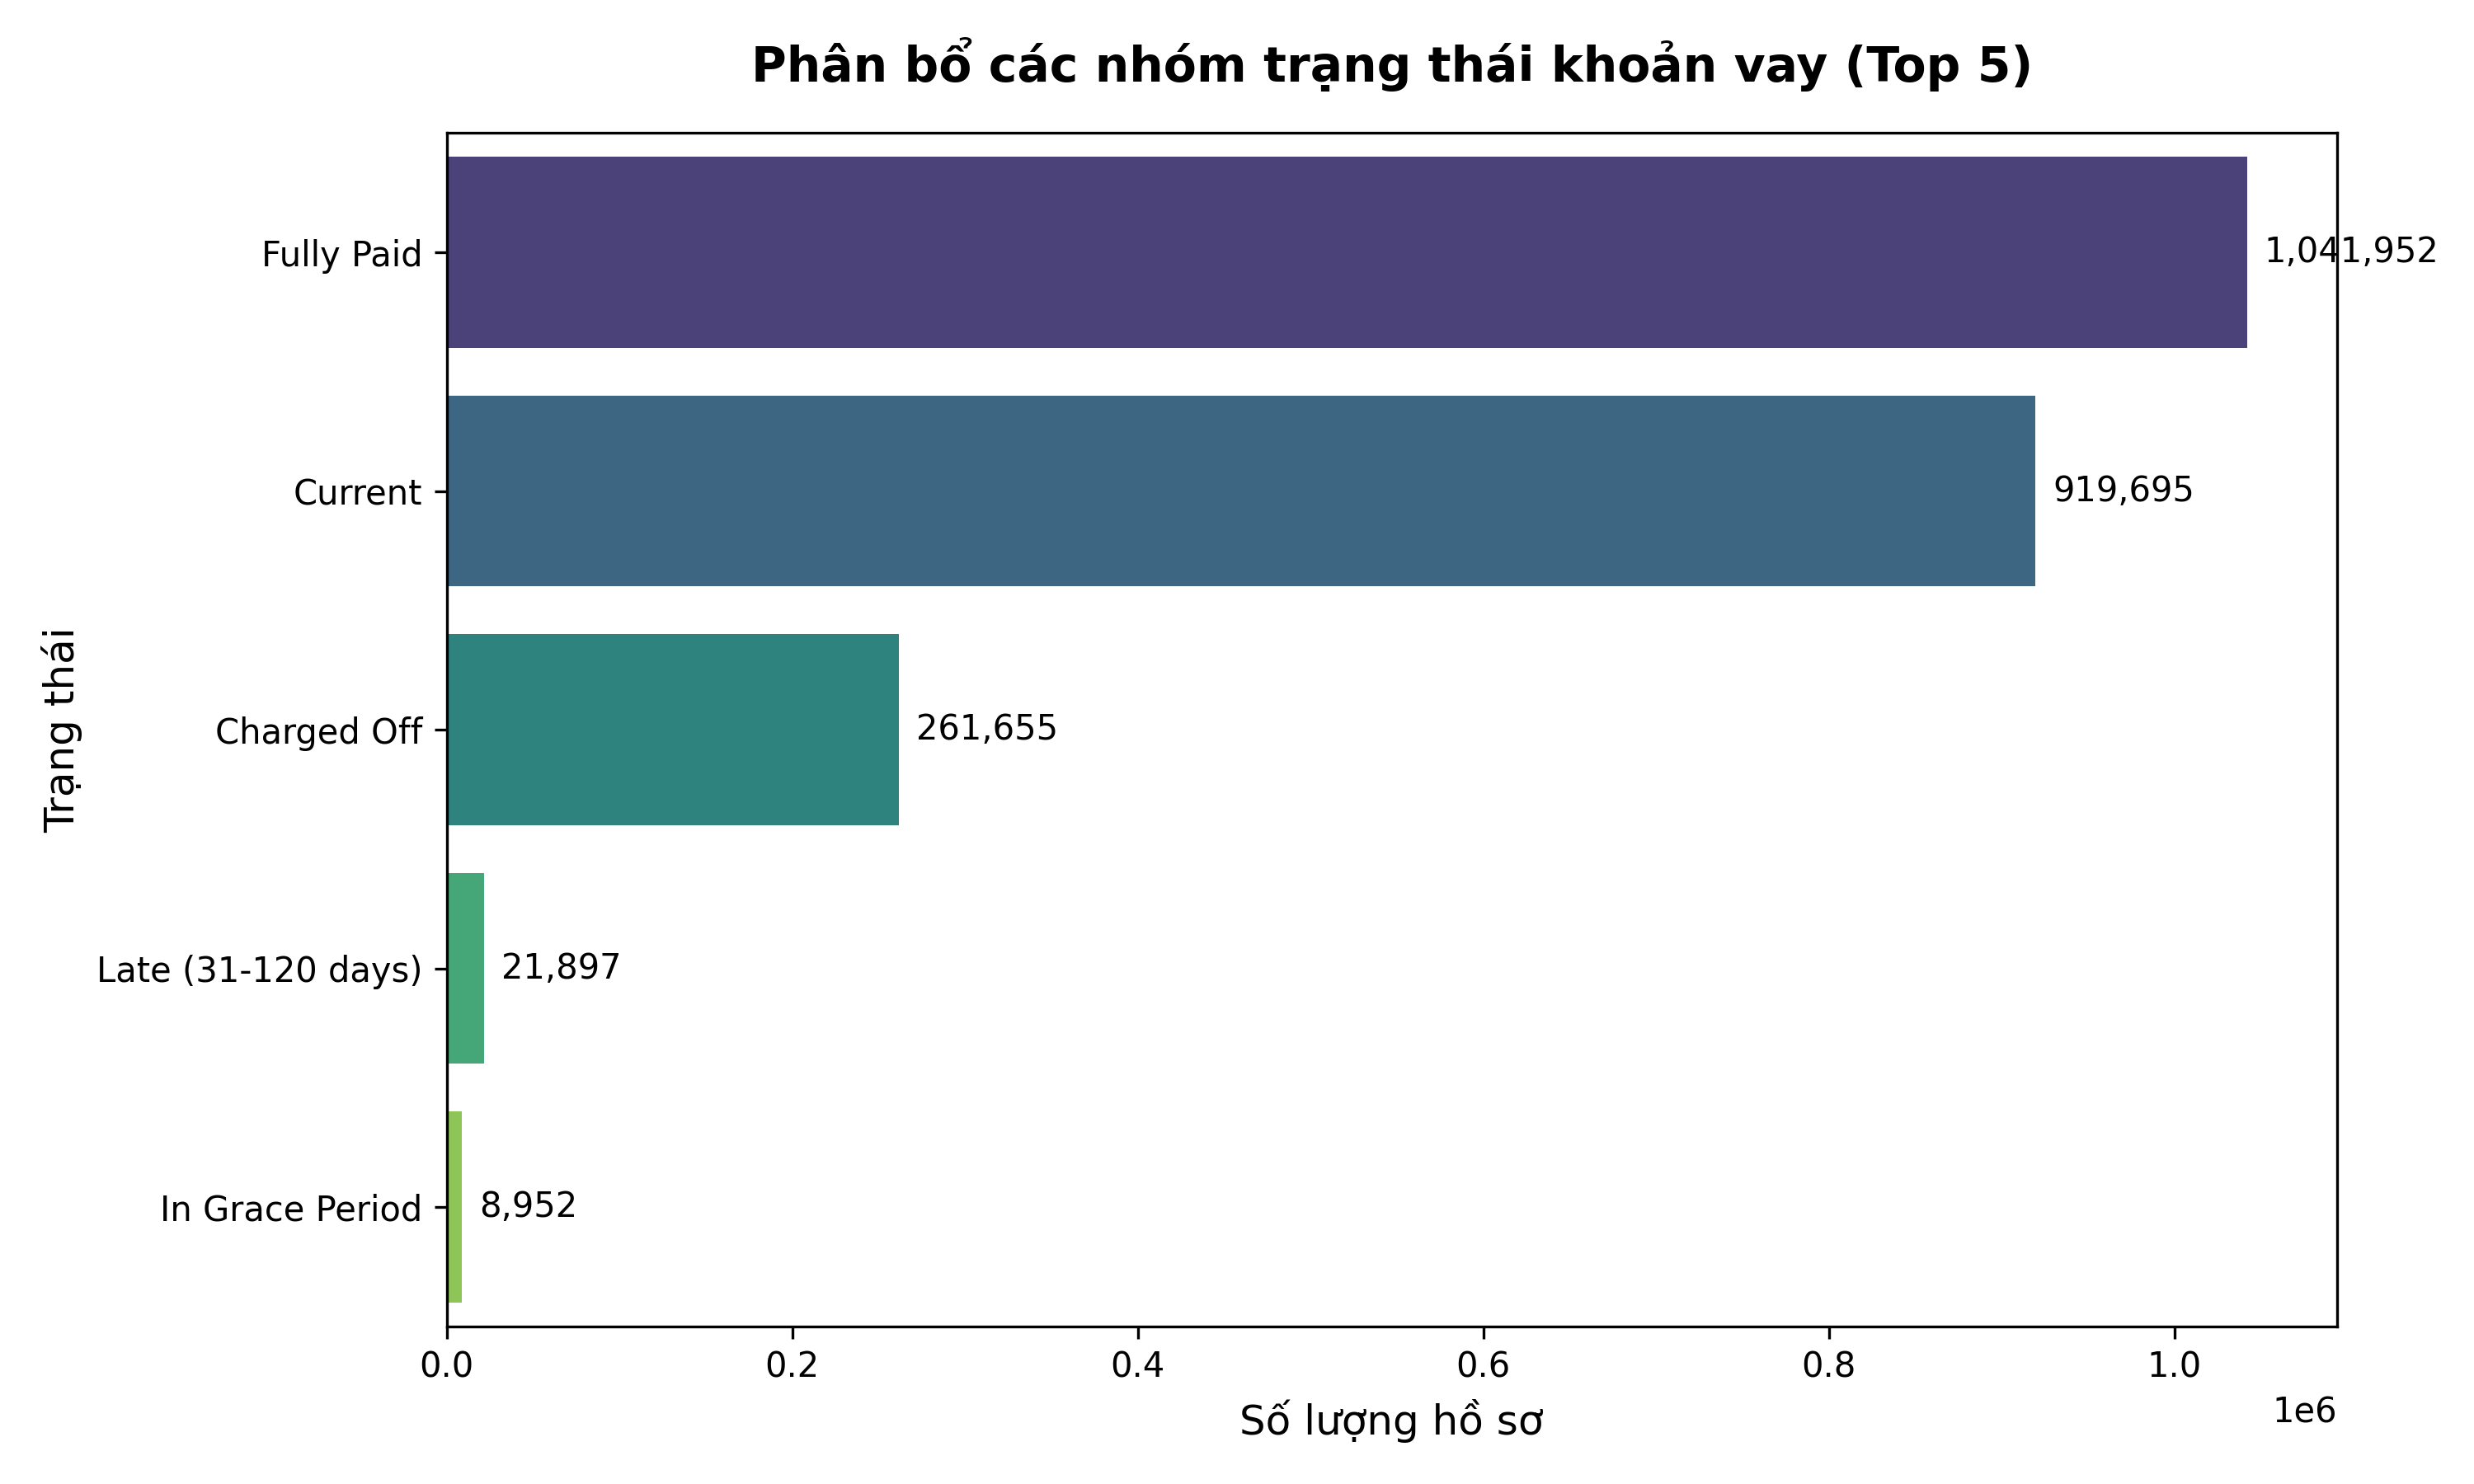
\includegraphics[width=0.75\textwidth]{images/0_loan_status_distribution.png}
    \caption{Phân bổ trạng thái khoản vay - Minh chứng cho sự mất cân bằng lớp}
    \label{fig:target_dist}
\end{figure}
\textit{Nhận xét:} Sự mất cân bằng này (Class Imbalance) là thách thức lớn; nếu không xử lý, mô hình sẽ có xu hướng luôn dự đoán khách hàng là "Tốt" để đạt độ chính xác ảo, dẫn đến rủi ro bỏ lọt nợ xấu cho ngân hàng.\\

\textbf{2. Tổng quan phân phối đặc trưng và Tỷ lệ khuyết thiếu (Hình \ref{fig:eda_grid})} \\
Lưới biểu đồ giúp quan sát hình dáng phân phối của 12 biến quan trọng. Đa số các biến định lượng như thu nhập (\texttt{annual\_inc}) đều bị lệch phải (right-skewed) rất nặng. 

\begin{figure}[H]
    \centering
    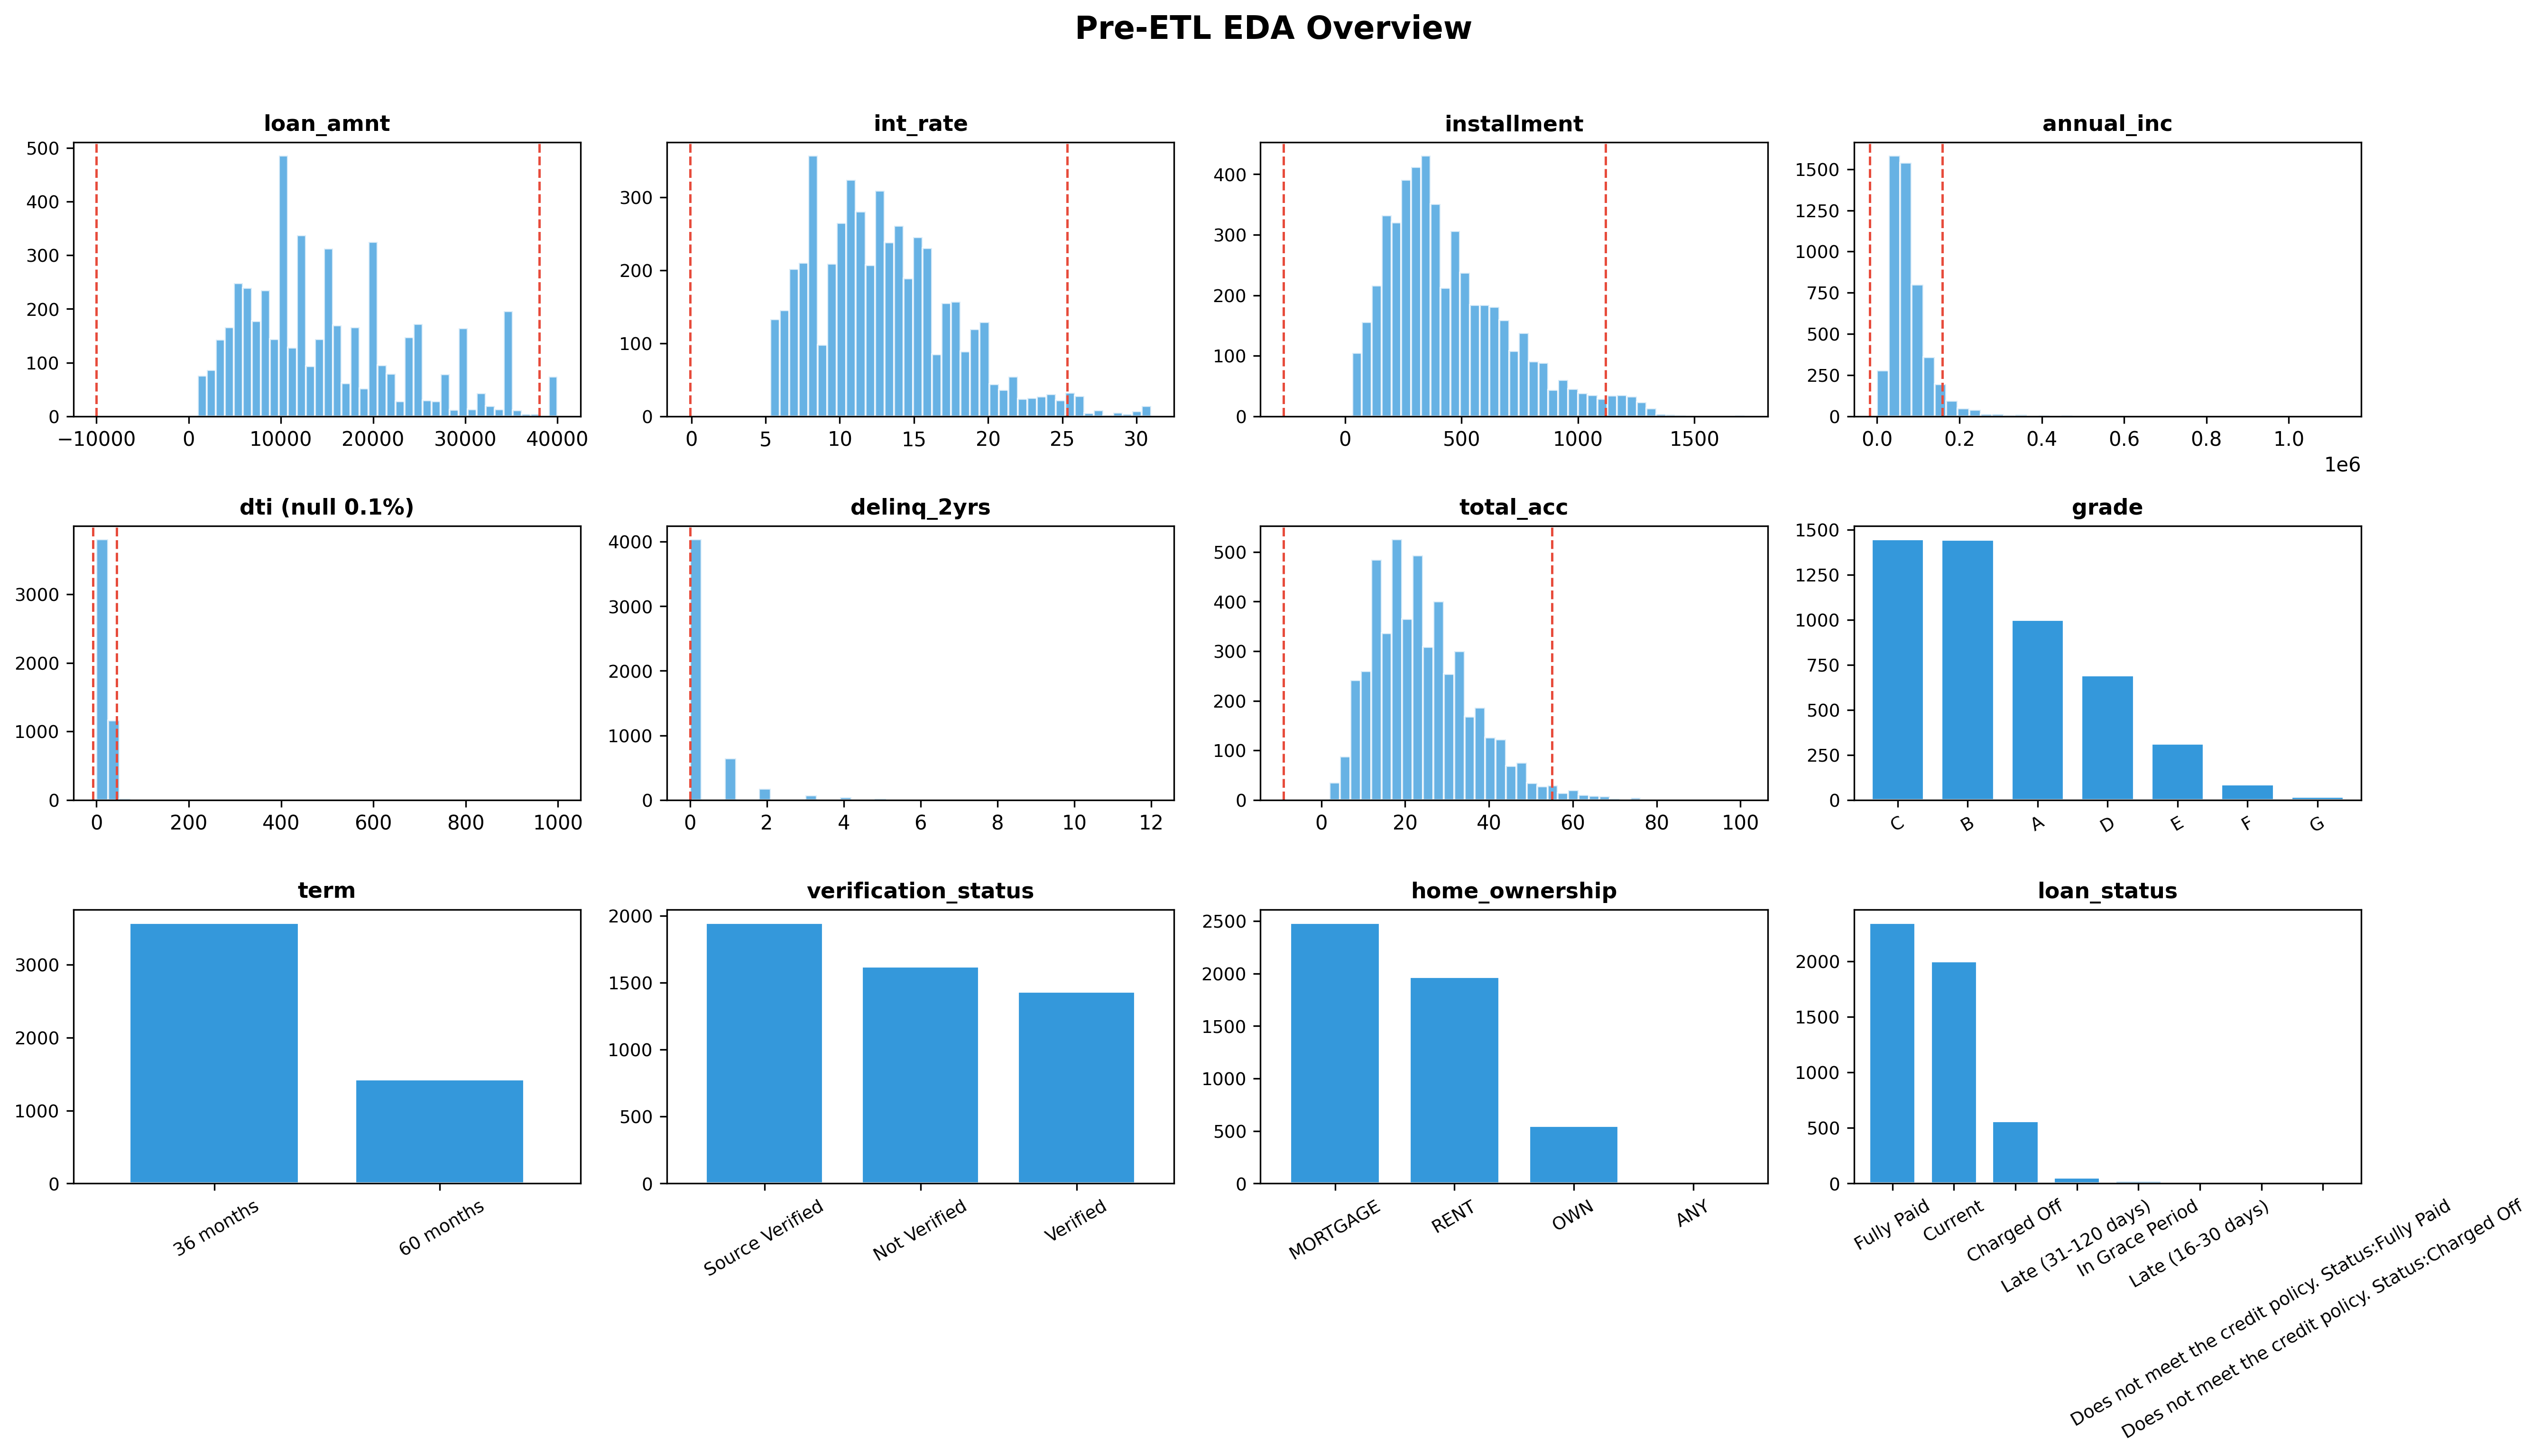
\includegraphics[width=0.95\textwidth]{images/1_pre_etl_eda_grid.png}
    \caption{Lưới phân phối đặc trưng và ghi chú tỷ lệ khuyết thiếu trực tiếp}
    \label{fig:eda_grid}
\end{figure}
\textit{Nhận xét:} Việc dữ liệu không phân phối chuẩn và có độ lệch cao yêu cầu nhóm phải áp dụng các kỹ thuật chuẩn hóa dữ liệu (\textit{Scaling/Transformation}) trước khi đưa vào huấn luyện AI.

\textbf{3. Rà soát điểm ngoại lệ theo nhóm trạng thái nợ (Hình \ref{fig:boxplot})} \\
Biểu đồ Boxplot so sánh sự khác biệt giữa các nhóm khách hàng. Có thể thấy rõ nhóm nợ xấu (\textit{Charged Off}) có xu hướng sở hữu mức lãi suất (\texttt{int\_rate}) cao hơn nhóm trả đủ. 

\begin{figure}[H]
    \centering
    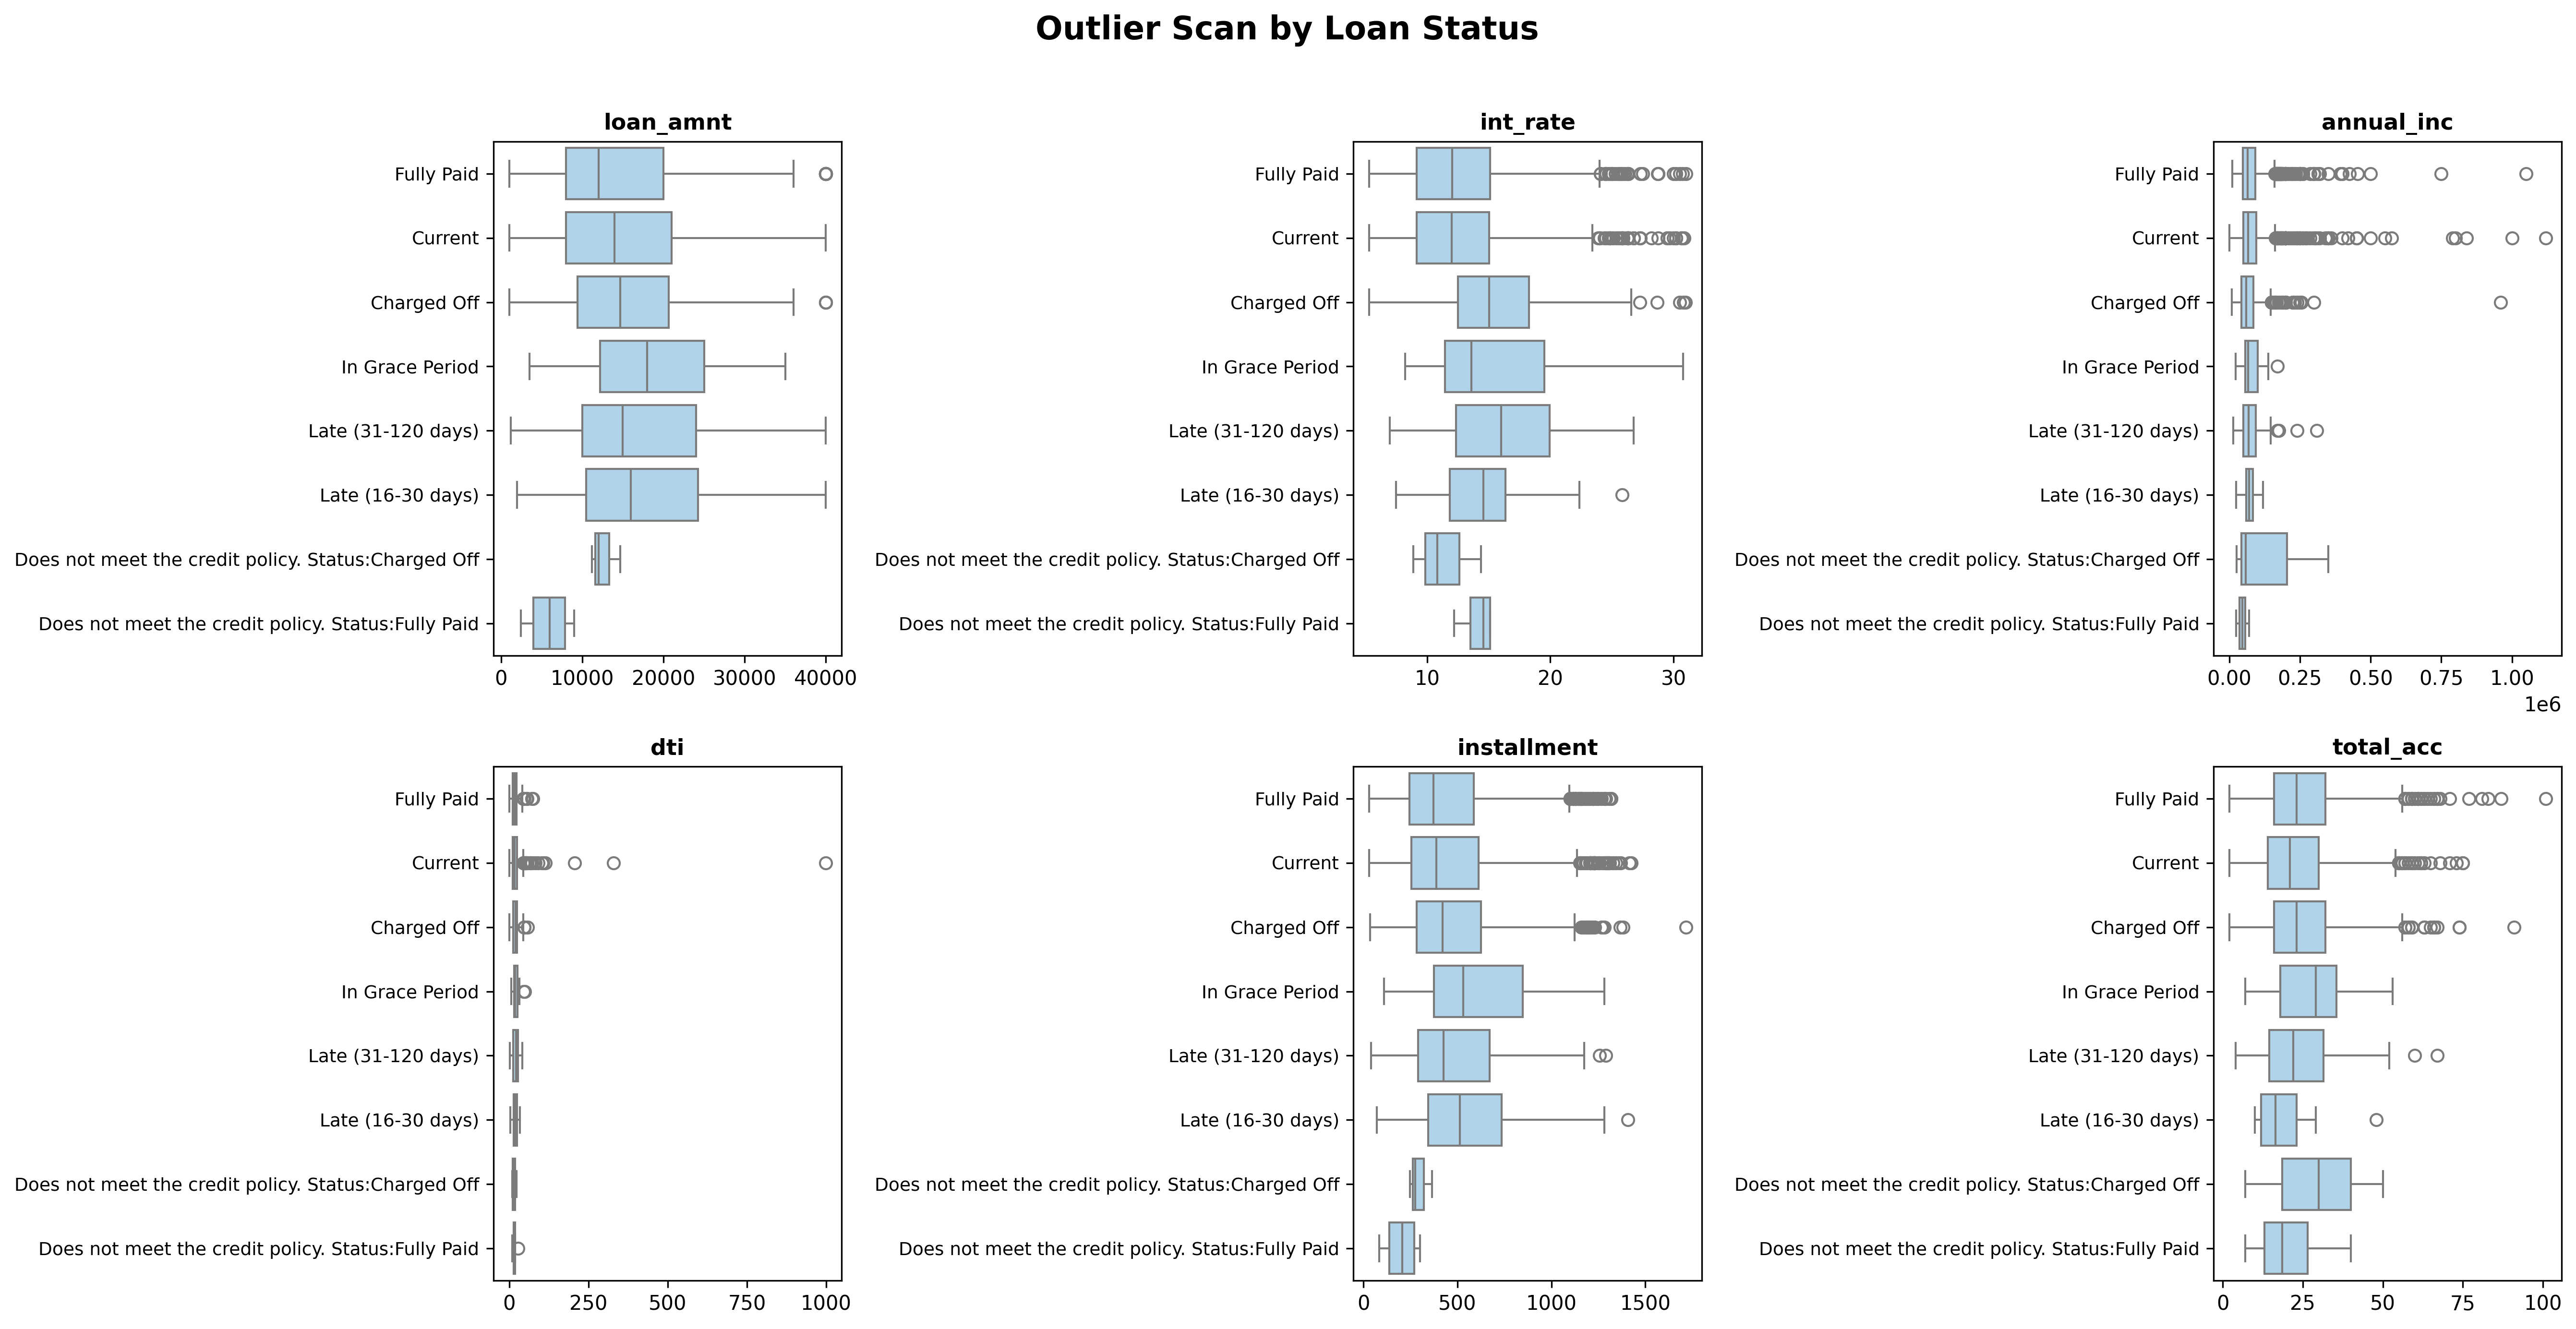
\includegraphics[width=0.95\textwidth]{images/2_boxplot_outlier.png}
    \caption{Phân tích điểm ngoại lệ và xu hướng lãi suất theo trạng thái nợ}
    \label{fig:boxplot}
\end{figure}
\textit{Nhận xét:} Sự hiện diện của các điểm ngoại lệ cực đoan (dấu chấm kéo dài) ở biến thu nhập cho thấy có những hồ sơ sở hữu giá trị thu nhập cực lớn so với phần lớn dân số vay vốn. Đây là các đối tượng cần được xử lý bằng phương pháp cắt ngọn hoặc chặn ngưỡng (\textit{Outlier Clipping}) để đảm bảo tính ổn định cho thuật toán.\\

\textbf{4. Ma trận tương quan xác định đặc trưng cốt lõi (Hình \ref{fig:heatmap})} \\

Ma trận tương quan Pearson được sử dụng để đánh giá mức độ liên hệ tuyến tính giữa các đặc trưng số và biến mục tiêu \texttt{loan\_status\_bin}. 

Đối với biến kỳ hạn khoản vay (\texttt{term}), dữ liệu gốc ở dạng chuỗi ký tự (ví dụ: “36 months”, “60 months”) đã được chuyển đổi sang dạng số (\texttt{term\_numeric}) nhằm phục vụ quá trình phân tích tương quan.

Kết quả cho thấy biến lãi suất (\texttt{int\_rate}) có mức tương quan dương cao nhất với biến mục tiêu, cho thấy các khoản vay có lãi suất cao thường đi kèm mức độ rủi ro tín dụng lớn hơn. Tuy nhiên, đa số các đặc trưng còn lại chỉ có hệ số tương quan thấp, phản ánh tính phức tạp của bài toán dự báo nợ xấu trong thực tế.

Ngoài ra, hai biến \texttt{loan\_amnt} và \texttt{installment} có hệ số tương quan rất cao (0.94), phản ánh hiện tượng đa cộng tuyến do khoản thanh toán hàng tháng phụ thuộc trực tiếp vào số tiền vay.

\begin{figure}[H]
    \centering
    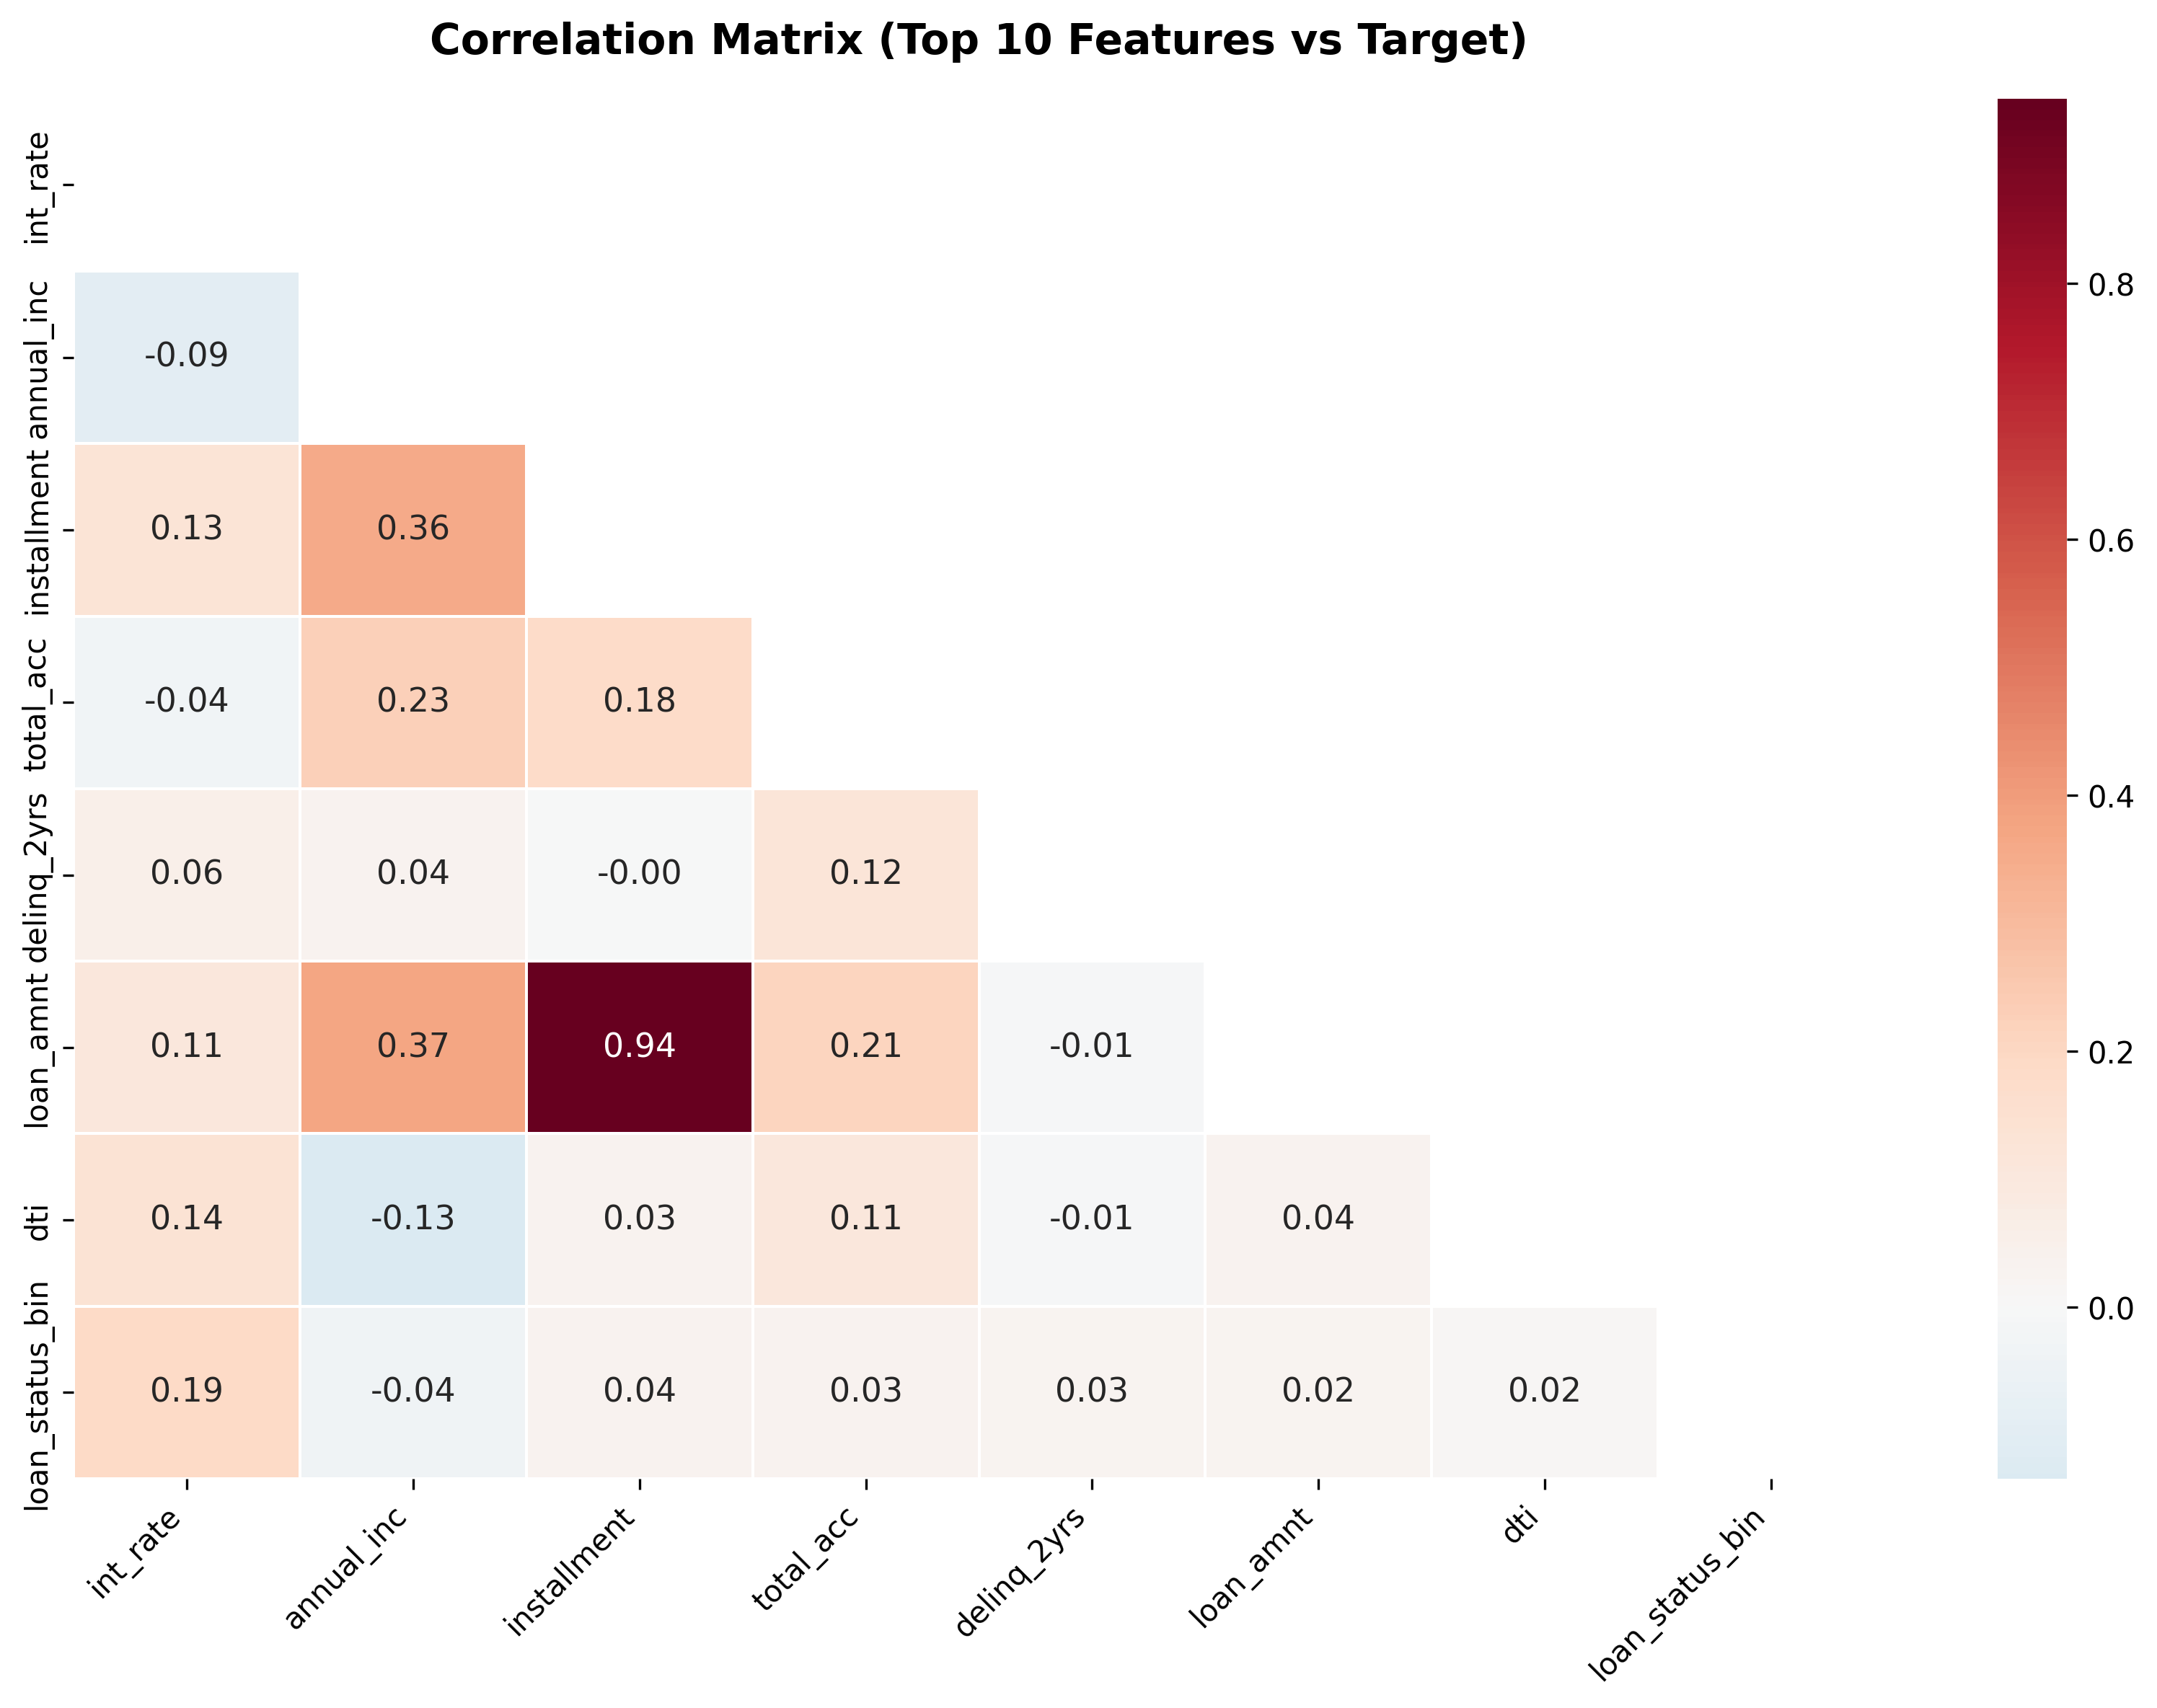
\includegraphics[width=0.75\textwidth]{images/3_correlation_matrix.png}
    \caption{Ma trận tương quan giữa các đặc trưng và biến mục tiêu}
    \label{fig:heatmap}
\end{figure}

\textit{Nhận xét:} Heatmap giúp xác định các đặc trưng mang tín hiệu dự báo tốt cho bài toán phân loại nợ xấu. Những biến có tương quan rất thấp với biến mục tiêu có thể được cân nhắc loại bỏ nhằm giảm độ phức tạp mô hình và chi phí tính toán, đặc biệt đối với các mô hình tuyến tính. Tuy nhiên điều này còn phụ thuộc vào loại mô hình học máy được sử dụng (các mô hình dạng cây quyết định - tree-based models vẫn có thể tận dụng tốt các đặc trưng này).

\subsection{Tiền xử lý và Làm sạch dữ liệu (Data Preprocessing \& Cleaning)}

Dữ liệu được tách thành hai nhánh rõ ràng theo nghiệp vụ.
Hệ thống áp dụng hai chiến lược gán nhãn khác nhau tùy theo mục đích sử dụng:
\begin{itemize}
    \item \textbf{Đối với nhánh AI:} Nhóm thực hiện loại bỏ các trạng thái trung gian như \textit{Late} hoặc \textit{In Grace Period}. Mục đích là để mô hình chỉ học từ các kết quả cuối cùng xác thực (\textit{Fully Paid} hoặc \textit{Charged Off}), từ đó đảm bảo độ ổn định và tránh nhiễu nhãn (label noise) trong quá trình huấn luyện.
    \item \textbf{Đối với nhánh BI (SQL Server):} Logic gán nhãn được thiết lập theo nguyên tắc quản trị rủi ro thận trọng. Các khoản vay trễ hạn (\textit{Late}) được ghi nhận là nhóm rủi ro (nhãn 1) trên Dashboard. Điều này giúp bộ phận quản lý nợ có cái nhìn tổng quát về các khoản nợ có vấn đề hiện tại để đưa ra quyết định xử lý kịp thời.
\end{itemize}


Các chiến lược xử lý chính bao gồm:

\begin{enumerate}
    \item \textbf{Khắc phục lỗi logic tài chính:} Loại bỏ các quan trắc vi phạm ràng buộc nghiệp vụ ($\texttt{annual\_inc} \le 0$, $\texttt{dti} < 0$, $\texttt{loan\_amnt} \le 0$, $\texttt{installment} \le 0$).
    \item \textbf{Loại bỏ bản ghi trùng lặp:} Kiểm tra và loại bỏ các dòng trùng hoàn toàn trên tập 13 biến trọng yếu bằng \texttt{drop\_duplicates()}.
    \item \textbf{Xử lý dữ liệu khuyết (Missing Values):}
    \begin{itemize}
        \item Điền giá trị ``Unknown'' cho trường \texttt{emp\_length} (thâm niên công tác).
        \item Loại bỏ các dòng thiếu ở các biến tài chính cốt lõi (\texttt{dti}, \texttt{annual\_inc}, \texttt{delinq\_2yrs}, \texttt{total\_acc}) — tỷ lệ rất thấp.
    \end{itemize}
    \item \textbf{Target Engineering:} Chỉ giữ hồ sơ đã đóng, tạo nhãn nhị phân \texttt{loan\_status\_bin} (Bad = 1, Good = 0).
    \item \textbf{Feature Engineering:} Số hóa biến \texttt{term} thành \texttt{term\_numeric}; cắt ngọn (clip) biến \texttt{annual\_inc} và \texttt{dti} tại phân vị 99\% để loại bỏ ngoại lệ cực đoan.
    \item \textbf{Giảm đa cộng tuyến:} Loại bỏ \texttt{installment} và \texttt{term} (chỉ áp dụng cho nhánh AI), đồng thời loại bỏ các biến gây rò rỉ dữ liệu (data leakage) như \texttt{recoveries}, \texttt{total\_pymnt}, \texttt{last\_pymnt\_amnt}, v.v.
\end{enumerate}

\begin{lstlisting}[language=Python, caption=Data Cleaning and Transformation Process (Excerpt)]
# 1. Financial logic validation
mask = pd.Series(True, index=df_bi.index)

if 'annual_inc' in df_bi.columns:
    mask &= df_bi['annual_inc'] > 0

if 'dti' in df_bi.columns:
    mask &= df_bi['dti'] >= 0

df_bi = df_bi[mask].copy()

# 2. Remove duplicate records
df_bi = df_bi.drop_duplicates().copy()

# 3. Handle missing values
df_bi['emp_length'] = df_bi['emp_length'].fillna('Unknown')

df_bi = df_bi.dropna(
    subset=['dti', 'annual_inc', 'delinq_2yrs', 'total_acc']
)

# 4. Create AI branch (closed loans only)
good_statuses = [
    'Fully Paid',
    'Does not meet the credit policy. Status:Fully Paid'
]

bad_statuses = [
    'Charged Off',
    'Default',
    'Does not meet the credit policy. Status:Charged Off'
]

df_clean = df_bi[
    df_bi['loan_status'].isin(good_statuses + bad_statuses)
].copy()

df_clean['loan_status_bin'] = (
    df_clean['loan_status'].isin(bad_statuses).astype(int)
)

# 5. Feature engineering
df_clean['term_numeric'] = (
    df_clean['term'].str.extract(r'(\d+)').astype(float)
)

INC_P99 = df_clean['annual_inc'].quantile(0.99)

df_clean['annual_inc_clipped'] = (
    df_clean['annual_inc'].clip(upper=INC_P99)
)

DTI_P99 = df_clean['dti'].quantile(0.99)

df_clean['dti_clipped'] = (
    df_clean['dti'].clip(upper=DTI_P99)
)

# 6. Remove redundant and leakage-prone features
df_clean.drop(
    columns=['installment', 'term', 'annual_inc', 'dti'],
    inplace=True
)
\end{lstlisting}
\textbf{Kết quả sau khi làm sạch:}

\begin{table}[H]
    \centering
    \renewcommand{\arraystretch}{1.2}
    \begin{tabular}{|l|r|r|}
        \hline
        \textbf{Tập dữ liệu} & \textbf{Số dòng} & \textbf{Số cột} \\ \hline
        BI (giữ Current) & 2.258.913 & 13 \\ \hline
        AI (chỉ hồ sơ đã đóng) & 1.306.043 & 13 \\ \hline
    \end{tabular}
    \caption{Kích thước tập dữ liệu sau khi làm sạch}
    \label{tab:clean_data_size}
\end{table}

\textit{Nhận xét:} Quá trình làm sạch đã loại bỏ \textbf{1.725 dòng} có lỗi logic tài chính, \textbf{5 dòng} trùng lặp sau bước lọc logic và các dòng thiếu ở biến tài chính cốt lõi. Đối với nhánh AI, việc chỉ giữ hồ sơ đã đóng giúp mô hình học được tín hiệu rõ ràng giữa ``Bùng nợ'' và ``Trả nợ tốt'', tránh nhiễu từ các hồ sơ còn đang trong quá trình trả nợ.

Để tăng tính kiểm chứng của quy trình ETL, notebook cũng xuất file \texttt{data/processed/etl\_summary.csv}. File này ghi lại số dòng trước và sau từng bước xử lý, giúp đối chiếu trực tiếp giữa code, dữ liệu đầu ra và báo cáo.

\begin{table}[H]
    \centering
    \renewcommand{\arraystretch}{1.2}
    \begin{tabular}{|l|r|r|r|}
        \hline
        \textbf{Bước ETL} & \textbf{Trước xử lý} & \textbf{Sau xử lý} & \textbf{Số dòng loại bỏ} \\ \hline
        Extract 13 biến trọng yếu & 2.260.668 & 2.260.668 & 0 \\ \hline
        Kiểm tra logic tài chính & 2.260.668 & 2.258.943 & 1.725 \\ \hline
        Loại bản ghi trùng lặp & 2.258.943 & 2.258.938 & 5 \\ \hline
        Xử lý missing values & 2.258.938 & 2.258.913 & 25 \\ \hline
        Tạo nhánh AI theo business rule & 2.258.913 & 1.306.043 & 952.870 \\ \hline
        Feature engineering và kiểm soát leakage & 1.306.043 & 1.306.043 & 0 \\ \hline
    \end{tabular}
    \caption{Tóm tắt số dòng trước và sau từng bước ETL}
    \label{tab:etl_summary}
\end{table}

\subsection{Chiến lược Lấy mẫu Dữ liệu (Data Sampling Strategy)}

Để phục vụ đồng thời hai mục tiêu là phân tích BI và huấn luyện mô hình AI, dữ liệu được tách thành hai nhánh riêng biệt theo mục đích sử dụng.\\
Trong đề tài này, em sử dụng quy trình ETL lai (hybrid ETL). Python được dùng ở giai đoạn đầu để đọc dữ liệu gốc, chọn 13 biến trọng yếu, kiểm tra chất lượng dữ liệu và tạo các tập dữ liệu phù hợp với từng mục đích sử dụng. Cách tiếp cận này giúp giảm tải cho SQL Server vì bộ dữ liệu gốc có quy mô lớn với hơn 2,2 triệu bản ghi và 145 thuộc tính.

Sau đó, SQL Server tiếp tục đảm nhiệm vai trò tổ chức dữ liệu theo mô hình Data Warehouse. Cụ thể, dữ liệu phục vụ BI được nạp vào vùng staging, sau đó được biến đổi thành các bảng Dimension, Fact và View phục vụ Power BI. Do đó, bước xử lý bằng Python không thay thế vai trò của SQL Server, mà đóng vai trò chuẩn bị dữ liệu đầu vào ở mức kỹ thuật để quá trình nạp và xây dựng kho dữ liệu diễn ra ổn định hơn.
\subsubsection{Living Sample Dataset (Dùng cho Data Warehouse \& Power BI)}
\begin{itemize}
    \item \textbf{Nguyên tắc:} Lấy mẫu ngẫu nhiên (Random Sampling) nhưng giữ nguyên tỷ lệ phân phối tự nhiên của dữ liệu gốc.
    \item \textbf{Mục đích:} Khi nạp vào SQL Server và vẽ Dashboard Power BI, các biểu đồ phải phản ánh đúng thực tế kinh doanh (ví dụ: tỷ lệ nợ xấu thực tế $\approx$ 11\%).
    \item \textbf{Kỹ thuật:} Trích xuất ngẫu nhiên \textbf{100.000 dòng} từ 2,2 triệu dòng.
\end{itemize}

\subsubsection{Balanced Dataset (Dùng cho Model AI)}
Việc tách riêng tập dữ liệu cho AI là cần thiết vì mục tiêu của mô hình học máy khác với mục tiêu của Dashboard BI. Dashboard cần phản ánh phân phối kinh doanh tự nhiên, do đó sử dụng tập dữ liệu giữ nguyên tỷ lệ thực tế. Ngược lại, mô hình AI cần học được đặc điểm của lớp nợ xấu, trong khi dữ liệu gốc bị lệch mạnh về nhóm khoản vay tốt. Nếu sử dụng trực tiếp tập 100.000 dòng từ nhánh BI/DWH để huấn luyện, mô hình có nguy cơ thiên lệch về lớp đa số và dự đoán kém đối với nhóm nợ xấu.

Vì vậy, nhóm tạo riêng tập \texttt{balanced\_model\_20k.csv} với tỷ lệ 1 hồ sơ xấu và 3 hồ sơ tốt. Tập này chỉ phục vụ huấn luyện và kiểm thử mô hình AI, không được dùng để báo cáo tỷ lệ nợ xấu thực tế trên Dashboard.
\begin{itemize}
    \item \textbf{Nguyên tắc:} Lấy mẫu có chủ đích (Under-sampling) để cân bằng giữa nhóm Tốt và Xấu.
    \item \textbf{Mục đích:} Tránh hiện tượng mô hình AI bị ``thiên kiến'' (Bias) do dữ liệu gốc quá lệch về nhóm khách hàng tốt. Giúp AI học được đặc điểm của nhóm nợ xấu hiệu quả hơn.
    \item \textbf{Kỹ thuật:} Lấy \textbf{5.000 hồ sơ Xấu} và \textbf{15.000 hồ sơ Tốt} (Tỷ lệ 1:3), tổng cộng \textbf{20.000 bản ghi}.
    \item \textbf{Lưu ý diễn giải:} Đây là tập huấn luyện đã được cân bằng có chủ đích, \textbf{không phản ánh phân phối tự nhiên} của dữ liệu kinh doanh. Vì vậy, file \texttt{balanced\_model\_20k.csv} chỉ dùng cho huấn luyện và kiểm thử mô hình AI, không dùng để báo cáo tỷ lệ nợ xấu trên Dashboard/Power BI.
\end{itemize}

\begin{lstlisting}[language=Python, caption=Mã thực thi chiến lược lấy mẫu phân tầng]
# A. Living Sample (DWH/Power BI) - Giu Current
df_living = df_bi.sample(n=100000, random_state=42)
df_living.to_csv(processed_dir / 'living_sample_100k.csv', index=False)

# B. Balanced Dataset (AI Model) - Chi tu ho so da dong
n_bad_actual = min(5000, len(df_bad))
n_good_actual = min(n_bad_actual * 3, len(df_good))

sample_bad = df_bad.sample(n=n_bad_actual, random_state=42)
sample_good = df_good.sample(n=n_good_actual, random_state=42)
df_balanced = pd.concat([sample_bad, sample_good]).sample(frac=1, random_state=42)
df_balanced.to_csv(processed_dir / 'balanced_model_20k.csv', index=False)
\end{lstlisting}

\textit{Nhận xét:} Chiến lược Under-sampling được lựa chọn thay vì Over-sampling (SMOTE) vì tập dữ liệu gốc đủ lớn (hơn 1,3 triệu hồ sơ). Việc lấy mẫu với tỷ lệ 1:3 giúp mô hình vừa học được đặc điểm nhóm nợ xấu, vừa không bị mất quá nhiều thông tin từ nhóm đa số. Trong giai đoạn huấn luyện, mô hình vẫn sử dụng thêm \texttt{class\_weight='balanced'} để tăng mức phạt khi dự đoán sai lớp nợ xấu.

Notebook đồng thời xuất file \texttt{data/processed/sampling\_summary.csv} để ghi rõ mục đích của từng file đầu ra: \texttt{living\_sample\_100k.csv} phục vụ DWH/Power BI với phân phối tự nhiên, còn \texttt{balanced\_model\_20k.csv} phục vụ AI với phân phối đã điều chỉnh.

\subsection{Chuẩn bị Dữ liệu cho Mô hình Học máy (Data Preparation for ML)}

Bước này được áp dụng trên tập dữ liệu đã làm sạch dành riêng cho AI. Để tránh rò rỉ dữ liệu, notebook chỉ thực hiện chia train/test trên dữ liệu thô ở bước này; các thao tác mã hóa và chuẩn hóa được đặt bên trong \texttt{sklearn Pipeline}/\texttt{ColumnTransformer} và chỉ được \texttt{fit} trên tập Train.

\subsubsection{Mã hóa biến phân loại (Categorical Encoding)}
\begin{itemize}
    \item \textbf{Ordinal Encoding:} Dành cho biến \texttt{grade} (A $\rightarrow$ G chuyển thành 1 $\rightarrow$ 7), vì các hạng tín dụng có thứ tự tự nhiên.
    \item \textbf{One-Hot Encoding (OHE):} Dành cho \texttt{home\_ownership}, \texttt{verification\_status} và \texttt{emp\_length}. Sử dụng \texttt{drop='first'} và \texttt{handle\_unknown='ignore'} để tránh bẫy đa cộng tuyến và xử lý category mới khi triển khai app.
\end{itemize}

\subsubsection{Chia tập dữ liệu (Train/Test Split)}
Phân chia \textbf{80\% Huấn luyện} và \textbf{20\% Kiểm thử}. Thực hiện cắt lớp (\texttt{stratify}) theo biến mục tiêu để giữ vững tỷ lệ nợ xấu trong tập balanced. Nếu notebook được chạy từ bước ETL và còn \texttt{df\_clean} trong bộ nhớ, nhóm tách thêm một \textit{natural holdout} 20\% trước khi lấy mẫu balanced để kiểm tra mô hình trên phân phối tự nhiên hơn.

\subsubsection{Chuẩn hóa dữ liệu số (Z-score Scaling)}
Đưa các biến định lượng (\texttt{loan\_amnt}, \texttt{int\_rate}, \texttt{annual\_inc\_clipped}, \texttt{dti\_clipped}, \texttt{total\_acc}, \texttt{term\_numeric}) về phân phối chuẩn bằng \texttt{StandardScaler} trong pipeline Logistic Regression. Random Forest chỉ dùng bước encoding và không cần scaling biến số.

\begin{lstlisting}[language=Python, caption=Mã chuẩn bị dữ liệu và pipeline tiền xử lý]
from sklearn.model_selection import train_test_split
from sklearn.compose import ColumnTransformer
from sklearn.preprocessing import OneHotEncoder, OrdinalEncoder, StandardScaler
from sklearn.pipeline import Pipeline

# 1. Train/Test Split tren du lieu raw
X_train, X_test, y_train, y_test = train_test_split(
    X, y, test_size=0.2, random_state=42, stratify=y)

# 2. Preprocessing chi fit ben trong Pipeline tren X_train
preprocessor_lr = ColumnTransformer([
    ('grade', OrdinalEncoder(categories=[['A','B','C','D','E','F','G']],
                             handle_unknown='use_encoded_value',
                             unknown_value=-1), ['grade']),
    ('categorical', OneHotEncoder(drop='first', handle_unknown='ignore',
                                  sparse_output=False),
     ['home_ownership', 'verification_status', 'emp_length']),
    ('numeric', StandardScaler(),
     ['loan_amnt', 'int_rate', 'annual_inc_clipped',
      'dti_clipped', 'total_acc', 'term_numeric'])
], remainder='drop')

lr_model = Pipeline([
    ('preprocessor', preprocessor_lr),
    ('model', LogisticRegression(max_iter=1000,
                                 class_weight='balanced',
                                 random_state=42))
])
\end{lstlisting}

\textbf{Kết quả sau khi chuẩn bị:}

\begin{table}[H]
    \centering
    \renewcommand{\arraystretch}{1.2}
    \begin{tabular}{|l|r|r|}
        \hline
        \textbf{Tập dữ liệu} & \textbf{Số mẫu} & \textbf{Số đặc trưng} \\ \hline
        X\_train / y\_train & 16.000 & 11 raw features \\ \hline
        X\_test / y\_test & 4.000 & 11 raw features \\ \hline
        Sau preprocessing & -- & 25 features \\ \hline
    \end{tabular}
    \caption{Kích thước tập huấn luyện và kiểm thử}
    \label{tab:train_test_size}
\end{table}

\textit{Nhận xét:} Việc đưa encoding và scaling vào \texttt{Pipeline} giúp loại bỏ nguy cơ fit encoder/scaler trên toàn bộ dữ liệu trước khi split. Đồng thời, app có thể load trực tiếp \texttt{loan\_pipeline.pkl}, bảo đảm preprocessing khi dự đoán giống với lúc huấn luyện.

\subsection{Tóm tắt đáp ứng yêu cầu tiền xử lý}
Phần tiền xử lý đã đáp ứng các yêu cầu chính của bài toán Data Mining:
\begin{itemize}
    \item \textbf{Data cleaning:} xử lý missing values, loại lỗi logic tài chính, loại duplicate và chuẩn hóa nhãn thiếu \texttt{emp\_length}.
    \item \textbf{Data transformation:} tạo \texttt{loan\_status\_bin}, chuyển \texttt{term} thành \texttt{term\_numeric}, clipping \texttt{annual\_inc}/\texttt{dti}, encoding biến phân loại và scaling biến số.
    \item \textbf{Business logic:} tách riêng nhánh BI/DWH và nhánh AI; loại các khoản vay chưa đóng khỏi tập huấn luyện để tránh nhãn không chắc chắn.
    \item \textbf{Feature selection:} chọn 13 biến trọng yếu dựa trên nghiệp vụ tín dụng, tránh data leakage và kiểm tra thêm bằng correlation/feature importance.
\end{itemize}

\newpage
\section{Data Warehouse Design}

\subsection{Mục tiêu thiết kế}
Kho dữ liệu được xây dựng để phục vụ hai nhu cầu chính: phân tích kinh doanh bằng Power BI và lưu trữ dữ liệu khoản vay theo cấu trúc ổn định, dễ truy vấn. Luồng triển khai của phần này là:

\begin{center}
\texttt{living\_sample\_100k.csv} $\rightarrow$ \texttt{stg.Loan\_Raw} $\rightarrow$ \texttt{dw.Dim\_*} $\rightarrow$ \texttt{dw.Fact\_Loan}
\end{center}

File \texttt{living\_sample\_100k.csv} là đầu ra của bước ETL trong notebook, giữ phân phối tự nhiên của dữ liệu kinh doanh để các dashboard phản ánh đúng tỷ lệ thực tế. File này được nạp vào SQL Server bằng script \texttt{import\_to\_sql.py}, sau đó script \texttt{sql/loan\_db.sql} tạo staging schema, data warehouse schema và nạp dữ liệu vào các bảng theo mô hình sao.

\subsection{Logical Design: Star Schema}
Nhóm thiết kế Data Warehouse theo mô hình \textbf{Star Schema}. Mô hình này có một bảng fact trung tâm kết nối với các bảng dimension thông qua khóa ngoại.

\subsubsection{Grain của bảng Fact}
Grain của bảng \texttt{dw.Fact\_Loan} là:

\begin{quote}
Mỗi dòng trong \texttt{Fact\_Loan} đại diện cho một hồ sơ khoản vay hợp lệ sau khi loại bỏ trạng thái \textit{Current} và các lỗi logic tài chính.
\end{quote}

Các measure chính trong bảng fact gồm:
\begin{itemize}
    \item \texttt{loan\_amnt}: số tiền vay.
    \item \texttt{int\_rate}: lãi suất khoản vay.
    \item \texttt{installment}: khoản trả góp hàng tháng.
    \item \texttt{loan\_status\_bin}: nhãn rủi ro dùng cho phân tích, trong đó 0 là hồ sơ tốt và 1 là hồ sơ xấu/trễ hạn.
\end{itemize}

\subsubsection{Các bảng Dimension}
\begin{itemize}
    \item \textbf{\texttt{dw.Dim\_Borrower}:} mô tả đặc điểm người vay, gồm \texttt{emp\_length}, \texttt{home\_ownership}, \texttt{annual\_inc}, \texttt{income\_bin}, \texttt{dti}, \texttt{delinq\_2yrs}, \texttt{total\_acc}.
    \item \textbf{\texttt{dw.Dim\_Loan\_Info}:} mô tả đặc điểm khoản vay, gồm \texttt{term}, \texttt{grade}, \texttt{verification\_status}.
\end{itemize}

\textit{Ghi chú kỹ thuật:} \texttt{Dim\_Borrower} hiện chứa một số thuộc tính định lượng như \texttt{annual\_inc}, \texttt{dti} và \texttt{total\_acc}, nên dimension này có cardinality cao. Với phạm vi bài tập lớn, thiết kế này vẫn chấp nhận được vì giúp Power BI phân tích trực tiếp theo thông tin người vay. Để tối ưu hơn trong hệ thống sản xuất, có thể chuyển một phần biến định lượng sang bảng fact hoặc chỉ giữ các biến đã được phân thùng như \texttt{income\_bin}.

\begin{figure}[H]
    \centering
    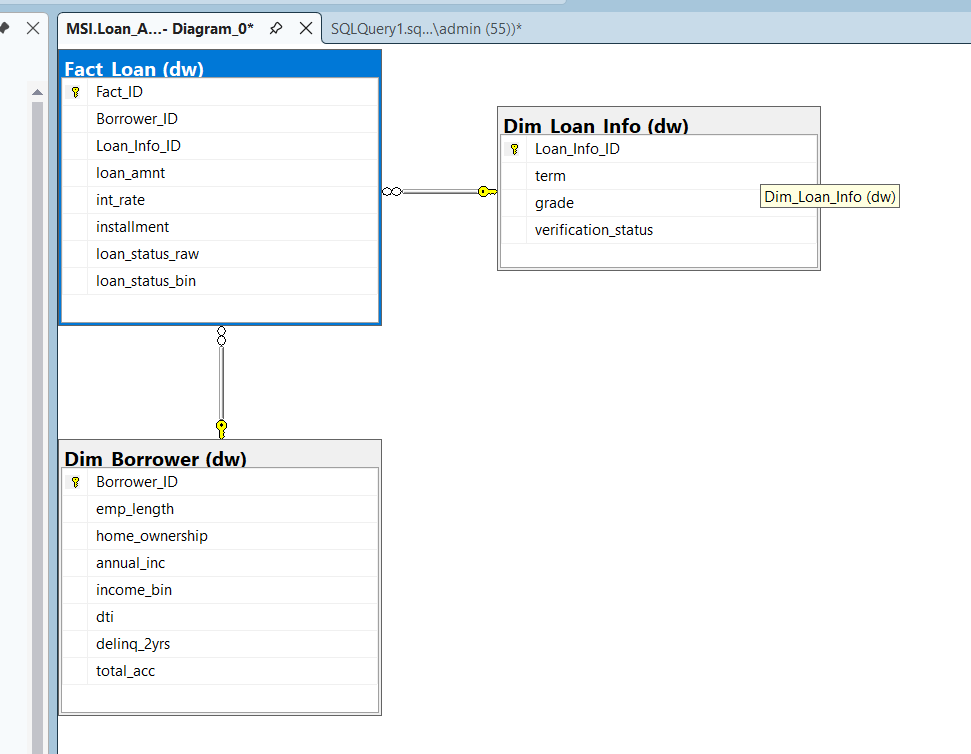
\includegraphics[width=0.8\textwidth]{images/Screenshot 2026-05-14 083154.png}
    \caption{Sơ đồ Star Schema của Data Warehouse khoản vay}
    \label{fig:star_schema}
\end{figure}

\subsection{Physical Design trên SQL Server}
Cấu trúc vật lý được chia thành hai schema:
\begin{itemize}
    \item \textbf{\texttt{stg}:} chứa bảng staging \texttt{stg.Loan\_Raw}, là nơi nhận dữ liệu từ file CSV.
    \item \textbf{\texttt{dw}:} chứa các bảng đã được tổ chức theo mô hình sao, gồm \texttt{dw.Dim\_Borrower}, \texttt{dw.Dim\_Loan\_Info} và \texttt{dw.Fact\_Loan}.
\end{itemize}

Script nạp dữ liệu \texttt{import\_to\_sql.py} ưu tiên đọc file \texttt{data/processed/living\_sample\_100k.csv}. Nếu file này chưa tồn tại, script mới dùng fallback là \texttt{data/raw/loan\_dw.csv}. Cách này đảm bảo nguồn nạp vào kho dữ liệu là output chính thức của bước ETL.

\subsection{ETL trong SQL Server}
Dựa trên file \texttt{sql/loan\_db.sql}, quá trình ETL trong SQL Server gồm ba bước:
\begin{enumerate}
    \item \textbf{Extract:} import CSV vào bảng \texttt{dbo.Loan\_Raw}, sau đó chuyển sang schema \texttt{stg}.
    \item \textbf{Transform:} lọc lỗi logic tài chính, loại trạng thái \textit{Current}, điền \texttt{Unknown} cho \texttt{emp\_length}, tạo \texttt{income\_bin} và chuyển \texttt{loan\_status} thành \texttt{loan\_status\_bin}.
    \item \textbf{Load:} nạp dữ liệu vào dimension trước, sau đó nạp fact bằng cách join với dimension để lấy surrogate key.
\end{enumerate}

\subsubsection{Business Logic trong SQL}
Các transformation quan trọng được thực hiện trực tiếp trong SQL:
\begin{itemize}
    \item \textbf{Data cleaning:} chỉ giữ hồ sơ có \texttt{annual\_inc > 0}, \texttt{dti >= 0}, \texttt{loan\_amnt > 0}, \texttt{installment > 0}; loại các dòng thiếu ở \texttt{delinq\_2yrs} và \texttt{total\_acc}.
    \item \textbf{Missing value handling:} chuyển \texttt{emp\_length} bị thiếu thành \texttt{Unknown}.
    \item \textbf{Data binning:} phân thùng \texttt{annual\_inc} thành \textit{Low Income}, \textit{Medium Income}, \textit{High Income}.
    \item \textbf{Target transformation:} chuyển \texttt{loan\_status} thành \texttt{loan\_status\_bin}. \textit{Fully Paid} và credit-policy fully paid được gán 0; \textit{Charged Off}, \textit{Default}, credit-policy charged off và các trạng thái \textit{Late} được gán 1.
\end{itemize}

\begin{lstlisting}[language=SQL, caption=Trích đoạn SQL tạo dimension và fact]
INSERT INTO dw.Dim_Borrower
    (emp_length, home_ownership, annual_inc, income_bin, dti, delinq_2yrs, total_acc)
SELECT DISTINCT
    ISNULL(CAST(emp_length AS NVARCHAR(50)), 'Unknown') AS emp_length,
    CAST(home_ownership AS NVARCHAR(50)),
    annual_inc,
    CASE
        WHEN annual_inc < 50000 THEN 'Low Income (<50k)'
        WHEN annual_inc >= 50000 AND annual_inc <= 100000 THEN 'Medium Income (50k-100k)'
        WHEN annual_inc > 100000 THEN 'High Income (>100k)'
        ELSE 'Unknown'
    END AS income_bin,
    dti, delinq_2yrs, total_acc
FROM stg.Loan_Raw
WHERE loan_status != 'Current'
  AND annual_inc > 0
  AND dti >= 0
  AND loan_amnt > 0
  AND installment > 0
  AND delinq_2yrs IS NOT NULL
  AND total_acc IS NOT NULL;

INSERT INTO dw.Fact_Loan
    (Borrower_ID, Loan_Info_ID, loan_amnt, int_rate, installment, loan_status_raw, loan_status_bin)
SELECT
    b.Borrower_ID,
    l.Loan_Info_ID,
    r.loan_amnt,
    r.int_rate,
    r.installment,
    r.loan_status,
    CASE
        WHEN r.loan_status IN ('Fully Paid',
             'Does not meet the credit policy. Status:Fully Paid') THEN 0
        WHEN r.loan_status IN ('Charged Off', 'Default',
             'Does not meet the credit policy. Status:Charged Off')
             OR r.loan_status LIKE '%Late%' THEN 1
        ELSE NULL
    END AS loan_status_bin
FROM stg.Loan_Raw r
JOIN dw.Dim_Borrower b
    ON ISNULL(CAST(r.emp_length AS NVARCHAR(50)), 'Unknown') = b.emp_length
    AND CAST(r.home_ownership AS NVARCHAR(50)) = b.home_ownership
    AND r.annual_inc = b.annual_inc
    AND r.dti = b.dti
    AND r.delinq_2yrs = b.delinq_2yrs
    AND r.total_acc = b.total_acc
JOIN dw.Dim_Loan_Info l
    ON CAST(r.term AS NVARCHAR(50)) = l.term
    AND CAST(r.grade AS NVARCHAR(50)) = l.grade
    AND CAST(r.verification_status AS NVARCHAR(50)) = l.verification_status
WHERE r.loan_status != 'Current'
  AND r.annual_inc > 0
  AND r.dti >= 0
  AND r.loan_amnt > 0
  AND r.installment > 0
  AND r.delinq_2yrs IS NOT NULL
  AND r.total_acc IS NOT NULL;
\end{lstlisting}

\subsection{Kiểm tra số dòng sau khi load}
Sau khi chạy \texttt{loan\_db.sql} trên file \texttt{living\_sample\_100k.csv}, số dòng kỳ vọng của các bảng như sau:

\begin{table}[H]
    \centering
    \renewcommand{\arraystretch}{1.2}
    \begin{tabular}{|l|r|l|}
        \hline
        \textbf{Bảng} & \textbf{Số dòng} & \textbf{Vai trò} \\ \hline
        \texttt{stg.Loan\_Raw} & 100.000 & Bảng staging nhận dữ liệu từ CSV \\ \hline
        \texttt{dw.Dim\_Borrower} & 59.314 & Dimension người vay \\ \hline
        \texttt{dw.Dim\_Loan\_Info} & 42 & Dimension thông tin khoản vay \\ \hline
        \texttt{dw.Fact\_Loan} & 59.337 & Fact khoản vay sau khi loại \textit{Current} và lỗi logic \\ \hline
    \end{tabular}
    \caption{Số dòng kỳ vọng sau khi load Data Warehouse}
    \label{tab:dwh_row_counts}
\end{table}

File SQL cũng có truy vấn kiểm tra cuối script để xác nhận số dòng thực tế sau khi load:

\begin{lstlisting}[language=SQL, caption=Truy vấn kiểm tra số dòng trong Data Warehouse]
SELECT 'stg.Loan_Raw' AS table_name, COUNT(*) AS row_count FROM stg.Loan_Raw
UNION ALL
SELECT 'dw.Dim_Borrower', COUNT(*) FROM dw.Dim_Borrower
UNION ALL
SELECT 'dw.Dim_Loan_Info', COUNT(*) FROM dw.Dim_Loan_Info
UNION ALL
SELECT 'dw.Fact_Loan', COUNT(*) FROM dw.Fact_Loan;
\end{lstlisting}

\begin{figure}[H]
    \centering
    \includegraphics[width=0.8\textwidth]{images/Screenshot 2026-05-16 135802.png} % Thay đổi tên file nếu cần
    \caption{Kết quả kiểm chứng dữ liệu sau quá trình ETL trong SQL Server}
    \label{fig:etl_results}
\end{figure}
Dựa trên Hình \ref{fig:etl_results}, kết quả thực thi các truy vấn kiểm tra cho thấy quá trình trích xuất và biến đổi dữ liệu (ETL) đã hoàn tất thành công. Cụ thể:
\begin{itemize}
    \item Tổng số dòng dữ liệu sạch được nạp vào bảng \textit{Fact\_Loan} là 59,337 dòng (đã loại bỏ các bản ghi không phù hợp).
    \item Biến mục tiêu (\textit{loan\_status\_bin}) đã được chuyển đổi chính xác sang dạng nhị phân: 0 (Nợ tốt) và 1 (Nợ xấu), sẵn sàng cho việc huấn luyện mô hình Machine Learning.
    \item Dữ liệu trong View \textit{vw\_Loan\_Dashboard} khớp hoàn toàn với bảng Fact, đảm bảo tính toàn vẹn dữ liệu cho báo cáo Power BI.
\end{itemize}

\newpage
\section{Trực quan hóa dữ liệu với Power BI}

\subsection{Mục tiêu Dashboard}
Sau khi xây dựng Data Warehouse trên SQL Server, nhóm kết nối Power BI trực tiếp đến schema \texttt{dw}. Dashboard được thiết kế để trả lời ba nhóm câu hỏi nghiệp vụ:
\begin{itemize}
    \item Quy mô danh mục khoản vay hiện tại là bao nhiêu?
    \item Nhóm khách hàng/khoản vay nào có tỷ lệ nợ xấu cao?
    \item Các đặc trưng như thu nhập, hạng tín dụng, kỳ hạn vay và tình trạng nhà ở ảnh hưởng đến rủi ro như thế nào?
\end{itemize}

Để thao tác Power BI đơn giản hơn, script SQL tạo thêm view \texttt{dw.vw\_Loan\_Dashboard}. View này nối sẵn \texttt{Fact\_Loan}, \texttt{Dim\_Borrower} và \texttt{Dim\_Loan\_Info}; vì vậy khi dựng dashboard, nhóm có thể kéo thả field từ một view duy nhất.

\subsection{Chuẩn bị dữ liệu trong Power BI}
\subsubsection{Kết nối dữ liệu}
Các bước kết nối:
\begin{enumerate}
    \item Chọn \textbf{Get Data} $\rightarrow$ \textbf{SQL Server}.
    \item Nhập server, ví dụ \texttt{localhost}, và database \texttt{Loan\_Approval\_DW}.
    \item Chọn view \texttt{dw.vw\_Loan\_Dashboard}. Nếu muốn trình bày mô hình sao, có thể chọn thêm \texttt{dw.Fact\_Loan}, \texttt{dw.Dim\_Borrower}, \texttt{dw.Dim\_Loan\_Info}.
    \item Chọn \textbf{Import} để dashboard chạy nhanh trên tập mẫu 100.000 dòng.
\end{enumerate}

\subsubsection{Các Measure DAX}
Nhóm tạo các measure chính sau trong Power BI:

\begin{lstlisting}[language=SQL, caption=Measure DAX sử dụng trong Dashboard]
Total Loans = COUNT('vw_Loan_Dashboard'[Fact_ID])

Bad Loans =
CALCULATE(
    COUNT('vw_Loan_Dashboard'[Fact_ID]),
    'vw_Loan_Dashboard'[loan_status_bin] = 1
)

Good Loans =
CALCULATE(
    COUNT('vw_Loan_Dashboard'[Fact_ID]),
    'vw_Loan_Dashboard'[loan_status_bin] = 0
)

Bad Loan Rate = DIVIDE([Bad Loans], [Bad Loans] + [Good Loans])

Average Loan Amount = AVERAGE('vw_Loan_Dashboard'[loan_amnt])

Average Interest Rate = AVERAGE('vw_Loan_Dashboard'[int_rate])
\end{lstlisting}

\textit{Lưu ý:} \texttt{Bad Loan Rate} không chia cho toàn bộ \texttt{Total Loans}, vì một số trạng thái như \textit{In Grace Period} có \texttt{loan\_status\_bin} rỗng. Công thức chỉ tính trên các hồ sơ đã có nhãn tốt/xấu rõ ràng.

\subsection{Thiết kế các biểu đồ chính}
\subsubsection{KPI Cards}
Phần đầu dashboard nên dùng các \textbf{Card Visuals} để hiển thị nhanh tình hình tổng quan:
\begin{itemize}
    \item \textbf{Total Loans:} tổng số khoản vay sau khi load vào fact.
    \item \textbf{Bad Loans:} số khoản vay rủi ro/nợ xấu.
    \item \textbf{Bad Loan Rate:} tỷ lệ nợ xấu trên các hồ sơ đã có nhãn tốt/xấu.
    \item \textbf{Average Loan Amount:} số tiền vay trung bình.
    \item \textbf{Average Interest Rate:} lãi suất trung bình.
\end{itemize}

\textbf{Cách làm trong Power BI:} chọn visual \textit{Card}, kéo từng measure vào ô \textit{Fields}. Với \texttt{Bad Loan Rate}, định dạng kiểu Percentage và làm tròn 1--2 chữ số thập phân.

\subsubsection{Biểu đồ 1: Phân bổ trạng thái khoản vay}
\begin{itemize}
    \item \textbf{Visual:} Clustered Bar Chart hoặc Donut Chart.
    \item \textbf{Axis/Legend:} \texttt{loan\_status\_raw}.
    \item \textbf{Values:} \texttt{Total Loans}.
\end{itemize}

\textbf{Ý nghĩa:} Biểu đồ này cho biết cơ cấu trạng thái khoản vay sau khi loại \textit{Current}. Nếu nhóm \textit{Fully Paid} chiếm đa số, danh mục có nhiều hồ sơ đã hoàn tất tốt. Các nhóm \textit{Charged Off}, \textit{Default} và \textit{Late} là vùng cần chú ý vì phản ánh rủi ro tín dụng.

\subsubsection{Biểu đồ 2: Histogram thu nhập khách hàng}
Theo yêu cầu đề bài, dashboard cần có biểu đồ histogram. Trong dự án này, nhóm tạo histogram bằng cột \texttt{income\_bin} đã được phân thùng trong SQL.

\begin{itemize}
    \item \textbf{Visual:} Clustered Column Chart.
    \item \textbf{X-axis:} \texttt{income\_bin}.
    \item \textbf{Y-axis:} \texttt{Total Loans}.
    \item \textbf{Format:} giảm \textit{Inner Padding} để các cột đứng gần nhau hơn.
\end{itemize}

\textbf{Cách kéo đúng:} không kéo \texttt{Fact\_ID} vào trục Y dưới dạng giá trị thô. Phải dùng measure \texttt{Total Loans = COUNT(Fact\_ID)} cho Y-axis, còn \texttt{income\_bin} nằm ở X-axis. Nếu kéo ngược lại, Power BI sẽ tạo một khối biểu đồ sai và không thể hiện được phân phối tần suất.

\textbf{Ý nghĩa:} Kết quả trên tập \texttt{living\_sample\_100k.csv} cho thấy nhóm \textit{Medium Income (50k--100k)} chiếm nhiều nhất, tiếp theo là \textit{Low Income (<50k)} và \textit{High Income (>100k)}. Điều này cho thấy danh mục vay tập trung chủ yếu ở nhóm thu nhập trung bình.

\begin{figure}[H]
    \centering
    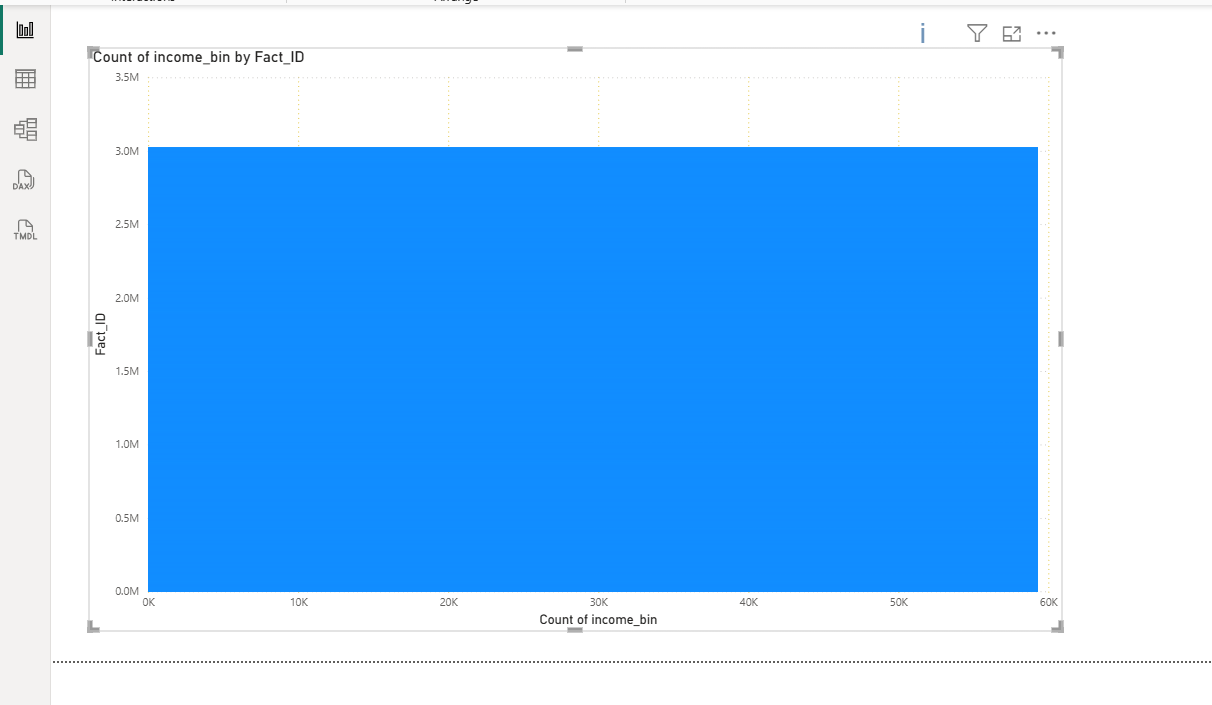
\includegraphics[width=0.75\textwidth]{images/Screenshot 2026-05-14 084744.png}
    \caption{Minh họa biểu đồ Histogram phân bổ khách hàng theo nhóm thu nhập}
    \label{fig:histogram_income}
\end{figure}

\subsubsection{Biểu đồ 3: Tỷ lệ nợ xấu theo hạng tín dụng}
\begin{itemize}
    \item \textbf{Visual:} Line and Clustered Column Chart hoặc Clustered Column Chart.
    \item \textbf{X-axis:} \texttt{grade}.
    \item \textbf{Column values:} \texttt{Total Loans}.
    \item \textbf{Line values:} \texttt{Bad Loan Rate}.
\end{itemize}

\textbf{Ý nghĩa:} Hạng tín dụng càng thấp thì rủi ro càng cao. Trên tập mẫu, tỷ lệ nợ xấu tăng dần từ nhóm A đến G: hạng A khoảng 6,7\%, hạng C khoảng 24,3\%, hạng E khoảng 39,4\% và hạng G hơn 51\%. Đây là insight quan trọng, chứng minh biến \texttt{grade} có ý nghĩa mạnh trong đánh giá rủi ro.

\subsubsection{Biểu đồ 4: Tỷ lệ nợ xấu theo kỳ hạn vay}
\begin{itemize}
    \item \textbf{Visual:} Clustered Column Chart.
    \item \textbf{X-axis:} \texttt{term}.
    \item \textbf{Y-axis:} \texttt{Bad Loan Rate}.
    \item \textbf{Tooltip:} \texttt{Total Loans}, \texttt{Average Interest Rate}.
\end{itemize}

\textbf{Ý nghĩa:} Khoản vay 60 tháng có tỷ lệ nợ xấu cao hơn khoản vay 36 tháng. Trên tập mẫu, nhóm 36 tháng có tỷ lệ nợ xấu khoảng 17,3\%, trong khi nhóm 60 tháng khoảng 34,0\%. Điều này phù hợp với nghiệp vụ tín dụng: kỳ hạn càng dài, rủi ro biến động thu nhập và khả năng trả nợ càng lớn.

\subsubsection{Biểu đồ 5: Tỷ lệ nợ xấu theo nhóm thu nhập}
\begin{itemize}
    \item \textbf{Visual:} Clustered Column Chart.
    \item \textbf{X-axis:} \texttt{income\_bin}.
    \item \textbf{Y-axis:} \texttt{Bad Loan Rate}.
\end{itemize}

\textbf{Ý nghĩa:} Nhóm \textit{Low Income} có tỷ lệ nợ xấu cao nhất, khoảng 24,0\%; nhóm \textit{Medium Income} khoảng 21,3\%; nhóm \textit{High Income} khoảng 17,6\%. Insight này cho thấy thu nhập thấp không chỉ làm giảm năng lực trả nợ mà còn là tín hiệu quan trọng trong phân tích rủi ro.

\subsubsection{Bộ lọc tương tác}
Dashboard nên có các slicer sau:
\begin{itemize}
    \item \texttt{grade}: lọc theo hạng tín dụng.
    \item \texttt{term}: lọc theo kỳ hạn vay.
    \item \texttt{home\_ownership}: lọc theo tình trạng nhà ở.
    \item \texttt{verification\_status}: lọc theo trạng thái xác minh thu nhập.
\end{itemize}

Các slicer giúp người dùng phân tích cùng một chỉ số dưới nhiều góc nhìn. Ví dụ, khi chọn riêng kỳ hạn 60 tháng, dashboard sẽ cho thấy nhóm nào có tỷ lệ nợ xấu cao hơn trong phân khúc vay dài hạn.

\subsection{Nhận xét tổng hợp}
Dashboard Power BI cho thấy ba insight chính:
\begin{enumerate}
    \item \textbf{Hạng tín dụng là biến phân tách rủi ro mạnh:} tỷ lệ nợ xấu tăng rõ rệt từ grade A đến G.
    \item \textbf{Kỳ hạn vay dài làm tăng rủi ro:} khoản vay 60 tháng có tỷ lệ nợ xấu gần gấp đôi khoản vay 36 tháng.
    \item \textbf{Thu nhập có liên hệ với khả năng trả nợ:} nhóm thu nhập thấp có tỷ lệ nợ xấu cao hơn nhóm thu nhập cao.
\end{enumerate}

Những insight này giúp bộ phận tín dụng điều chỉnh chính sách phê duyệt, chẳng hạn kiểm soát chặt hơn với khách hàng có grade thấp, kỳ hạn dài và thu nhập thấp.

\newpage
\section{Modeling \& Results}

\subsection{Machine Learning Algorithms}
Sau khi dữ liệu đã được tiền xử lý và xử lý mất cân bằng lớp bằng chiến lược under-sampling có chủ đích (tỷ lệ 1 nợ xấu : 3 trả tốt), nhóm tiến hành huấn luyện các thuật toán học máy để dự báo khả năng khách hàng vỡ nợ. Hai thuật toán đại diện cho hai trường phái khác nhau được lựa chọn để so sánh:

\begin{enumerate}
    \item \textbf{Logistic Regression (Hồi quy Logistic):} Đây là mô hình phân loại tuyến tính cổ điển. Ưu điểm lớn nhất của nó là \textit{khả năng giải thích (Interpretability)} cao. Trong lĩnh vực tài chính ngân hàng, việc có thể giải thích được lý do từ chối hay chấp nhận một khoản vay cho khách hàng là yêu cầu bắt buộc của các cơ quan quản lý. Thuật toán này đóng vai trò là mô hình cơ sở (Baseline Model).
    \item \textbf{Random Forest Classifier (Rừng ngẫu nhiên):} Một mô hình phi tuyến tính thuộc họ Ensemble Learning. Thuật toán hoạt động bằng cách xây dựng hàng loạt cây quyết định (Decision Trees) và tổng hợp kết quả của chúng. Random Forest nổi bật với khả năng nắm bắt các mối quan hệ phức tạp, tương tác chéo giữa các đặc trưng (features) và có khả năng chống hiện tượng học vẹt (Overfitting) rất tốt.
\end{enumerate}

\subsection{Model Training \& Tuning}
\subsubsection{Lựa chọn Metric Đánh giá (Evaluation Metrics)}
Trong bài toán tín dụng, một khách hàng bị phân loại nhầm thành "Nợ xấu" (False Positive) chỉ làm ngân hàng mất đi một khoản lãi suất tiềm năng. Tuy nhiên, nếu mô hình "bỏ lọt" một khách hàng thực sự vỡ nợ (False Negative), ngân hàng có nguy cơ mất trắng toàn bộ vốn gốc. 

Do đó, thay vì sử dụng độ chính xác tổng thể (Accuracy), nhóm ưu tiên hai độ đo sau:
\begin{itemize}
    \item \textbf{Recall (Độ phủ) của lớp Nợ xấu (Class 1):} Tỷ lệ nợ xấu thực tế được mô hình nhận diện thành công. Recall càng cao, số lượng nợ xấu bị bỏ lọt càng thấp.
    \item \textbf{ROC-AUC Score:} Thể hiện khả năng phân tách tổng quát của mô hình giữa hai lớp Tốt và Xấu ở nhiều ngưỡng xác suất khác nhau.
\end{itemize}

\subsubsection{Kết quả Huấn luyện Baseline}
Dữ liệu được chia thành tập Huấn luyện (Train) và tập Kiểm thử (Test) theo tỷ lệ 80/20, có \texttt{stratify} theo biến mục tiêu. Để tránh rò rỉ dữ liệu, nhóm đóng gói toàn bộ bước mã hóa và chuẩn hóa trong \texttt{sklearn Pipeline}: \texttt{OrdinalEncoder} cho \texttt{grade}, \texttt{OneHotEncoder} cho các biến danh mục, và \texttt{StandardScaler} cho các biến số trong pipeline Logistic Regression. Kết quả huấn luyện ban đầu trên 4.000 hồ sơ kiểm thử như sau:

\begin{itemize}
    \item \textbf{Logistic Regression:} Đạt ROC-AUC Score là \textbf{0.6847}. Recall cho lớp Nợ xấu đạt \textbf{0.61}.
    \item \textbf{Random Forest (Mặc định):} Đạt ROC-AUC Score là \textbf{0.6751}. Recall cho lớp Nợ xấu đạt \textbf{0.55}.
\end{itemize}
Có thể thấy ở thiết lập mặc định, Logistic Regression đang tỏ ra nhạy bén hơn trong việc bắt các ca nợ xấu (Recall 0.61 so với 0.55). Tuy nhiên, Random Forest là mô hình có rất nhiều siêu tham số, do đó nhóm tiến hành tối ưu hóa (Tuning).

\subsubsection{Tối ưu hóa siêu tham số (Hyperparameter Tuning)}
Nhóm áp dụng kỹ thuật \texttt{RandomizedSearchCV} trên không gian tham số của Random Forest để tìm ra cấu hình tốt nhất. 
\begin{lstlisting}[language=Python, caption=Tối ưu hóa tham số với RandomizedSearchCV]
# Best Params được tìm ra:
{'model__n_estimators': 100, 
 'model__min_samples_split': 2, 
 'model__min_samples_leaf': 1, 
 'model__max_depth': 5}
\end{lstlisting}

Sau khi tinh chỉnh, \textbf{Random Forest (Tuned)} đã ghi nhận sự cải thiện đáng kể:
\begin{itemize}
    \item \textbf{ROC-AUC Score:} Đạt \textbf{0.6774}.
    \item \textbf{Recall (Lớp 1 - Nợ xấu):} Tăng vọt từ 0.55 lên \textbf{0.68}.
\end{itemize}

Sự đánh đổi ở đây là độ chính xác tổng thể (Accuracy) giảm từ 0.66 xuống 0.60, đồng thời Precision của lớp nợ xấu chỉ đạt khoảng 0.34. Vì ROC-AUC của Logistic Regression cao hơn và mô hình này dễ giải thích hơn, nhóm chọn Logistic Regression Pipeline làm mô hình chính; Random Forest tuned được giữ như mô hình so sánh khi muốn ưu tiên Recall cao hơn.

\subsection{Evaluation Results \& Model Export}
\subsubsection{So sánh đường cong ROC (ROC Curve Comparison)}
Để đánh giá khả năng phân tách tổng quát giữa hai lớp Tốt/Xấu của các mô hình tại các ngưỡng (thresholds) xác suất khác nhau, nhóm sử dụng đường cong ROC. Biểu đồ \ref{fig:roc_compare} trình bày sự so sánh giữa đường cong ROC của mô hình Logistic Regression và mô hình Random Forest (sau khi đã tối ưu).

\begin{figure}[H]
    \centering
    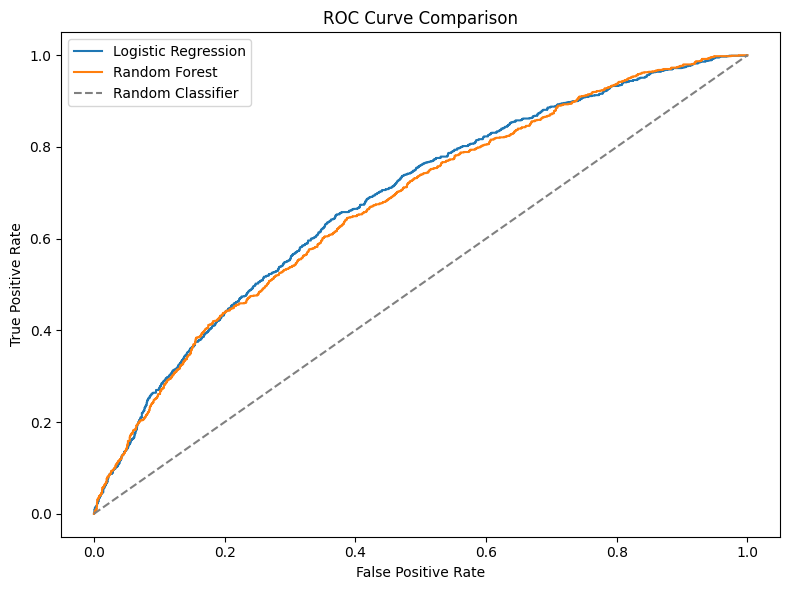
\includegraphics[width=0.8\textwidth]{images/outputroc.png} % Hãy lưu ảnh ROC Curve vào thư mục images với tên này
    \caption{Đường cong ROC so sánh Logistic Regression và Random Forest (Tuned)}
    \label{fig:roc_compare}
\end{figure}

\textit{Nhận xét:} Dựa trên biểu đồ và ROC-AUC, Logistic Regression có khả năng phân tách tổng quát nhỉnh hơn nhẹ so với Random Forest tuned trên tập kiểm thử balanced. Random Forest tuned có Recall lớp nợ xấu cao hơn, nhưng đánh đổi bằng nhiều dự đoán dương tính giả hơn. Vì vậy, Logistic Regression phù hợp hơn làm mô hình triển khai chính trong bối cảnh cần giải thích quyết định tín dụng.
\subsubsection{Đánh giá mức độ quan trọng của Đặc trưng (Feature Importance)}
Một trong những tính năng mạnh mẽ của Random Forest là khả năng trích xuất độ quan trọng của các biến đầu vào. Kết quả (Hình \ref{fig:feature_importance}) cho thấy Top 3 yếu tố quyết định lớn nhất đến khả năng vỡ nợ của một khách hàng bao gồm:
\begin{enumerate}
    \item Lãi suất (\texttt{int\_rate}) - Trọng số: 0.205
    \item Hạng tín dụng (\texttt{grade}) - Trọng số: 0.199
    \item Tỷ lệ nợ trên thu nhập (\texttt{dti\_clipped}) - Trọng số: 0.125
\end{enumerate}

\begin{figure}[H]
    \centering
    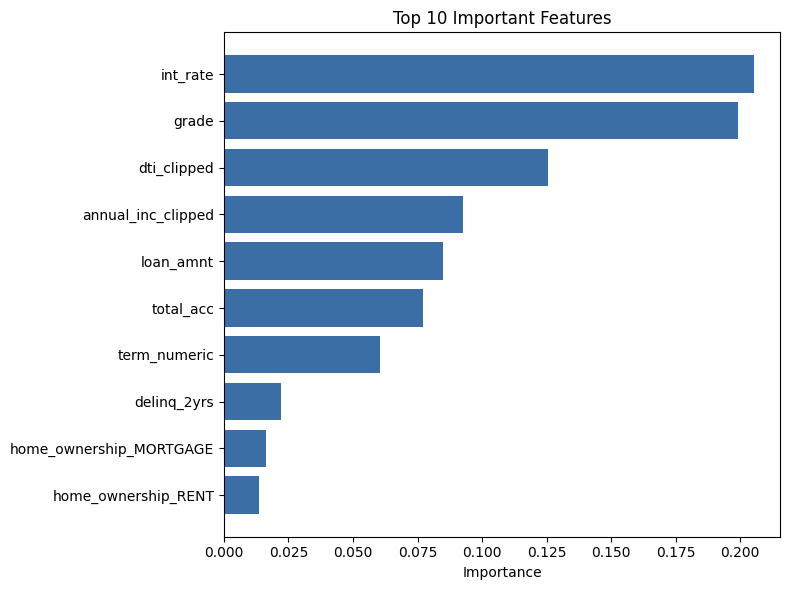
\includegraphics[width=0.8\textwidth]{images/outputfu.png} % Hãy lưu ảnh Feature Importance vào thư mục images với tên này
    \caption{Mức độ quan trọng của các đặc trưng (Top 10 Feature Importance)}
    \label{fig:feature_importance}
\end{figure}

\begin{figure}[H]
    \centering
    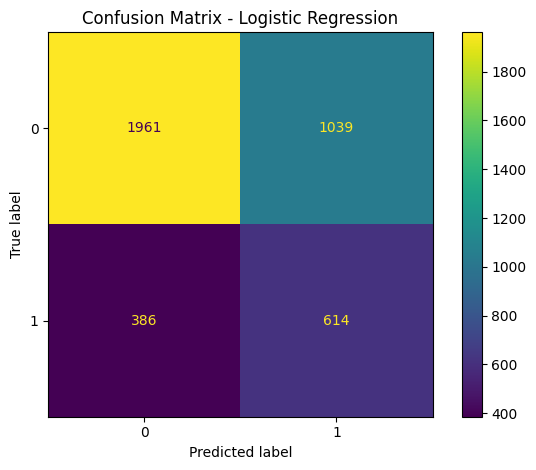
\includegraphics[width=0.8\textwidth]{images/outputcon.png} % Hãy lưu ảnh Confusion Matrix vào thư mục images với tên này
    \caption{Ma trận nhầm lẫn (Confusion Matrix) của Random Forest và Logistic Regression}
    \label{fig:confusion_matrix}
\end{figure}

\subsubsection{Trích xuất và Triển khai Mô hình (Model Export)}
Kết thúc quá trình phân tích, để chuẩn bị cho việc xây dựng ứng dụng hoặc tích hợp vào hệ thống máy chủ, nhóm đã tiến hành đóng gói (serialize) toàn bộ quy trình bằng \texttt{joblib} và \texttt{json}. 

Hệ thống đã lưu trữ thành công các cấu phần cốt lõi tại thư mục \texttt{/app/models/}:
\begin{itemize}
    \item Pipeline mô hình chính: \texttt{loan\_pipeline.pkl} (preprocessing + Logistic Regression).
    \item Mô hình so sánh: \texttt{rf\_tuned\_pipeline.pkl} (preprocessing + Random Forest tuned).
    \item Artifact tương thích: \texttt{lr\_model.pkl} và \texttt{preprocessor\_lr.pkl}.
    \item Cấu hình đặc trưng: \texttt{model\_input\_features.json}, \texttt{feature\_names.json} (25 features sau preprocessing) và \texttt{clip\_params.json}.
\end{itemize}
Bộ hồ sơ triển khai này đảm bảo rằng khi một dòng dữ liệu khách hàng mới (thô) được truyền vào, hệ thống sẽ tự động áp dụng đúng clipping, encoding và scaling đã học từ tập Train trước khi mô hình đưa ra phán quyết cuối cùng.

\newpage
\section{Hệ thống Web App Hỗ trợ Ra quyết định (Streamlit \& FastAPI)}

Trong giai đoạn cuối cùng của dự án, mô hình Machine Learning sau khi huấn luyện thành công đã được tích hợp vào một hệ thống Web Application hoàn chỉnh, đóng vai trò là một Hệ Hỗ trợ Ra Quyết định (Decision Support System - DSS) thực thụ cho các nhân viên tín dụng. Hệ thống đã được xây dựng và triển khai thực tế với kiến trúc Microservices cơ bản, bao gồm 3 thành phần chính:

\begin{itemize}
    \item \textbf{Frontend (Streamlit - Port 8501):} Giao diện người dùng được xây dựng bằng framework Streamlit, cung cấp một Dashboard tương tác trực quan, hiện đại (Dark Theme). Nhân viên tín dụng điền các thông tin thô của hồ sơ vay (số tiền, lãi suất, hạng tín dụng, v.v.) thông qua các Form thân thiện. Hệ thống tích hợp biểu đồ Gauge hiển thị trực quan mức độ rủi ro (Risk Probability).
    \item \textbf{Backend (FastAPI - Port 8000):} Xây dựng bằng FastAPI chuẩn RESTful API. Backend tiếp nhận dữ liệu, tự động chạy qua đường ống tiền xử lý (Clipping, Encoding, Scaling) hoàn toàn giống với lúc huấn luyện, sau đó đưa vào mô hình Logistic Regression để đưa ra dự đoán.
    \item \textbf{Database (PostgreSQL - Port 5432):} Tích hợp SQLAlchemy ORM để tự động lưu vết (logging) toàn bộ lịch sử các lượt thẩm định vào bảng \texttt{loan\_predictions}, phục vụ công tác kiểm toán và tái huấn luyện mô hình.
\end{itemize}

\subsection{Kịch bản Thực nghiệm Hệ thống (System Testing)}
Để minh họa khả năng hoạt động của hệ thống, nhóm trình bày hai kịch bản thẩm định đối lập dựa trên dữ liệu thực tế:

\subsubsection{Kịch bản 1: Phê duyệt hồ sơ rủi ro thấp}
\begin{itemize}
    \item \textbf{Dữ liệu đầu vào:} Số tiền vay: \$10,000 | Lãi suất: 7.5\% | Hạng tín dụng: A | Thu nhập: \$120,000 | DTI: 8\% | Trễ hạn: 0.
    \item \textbf{Kết quả trả về:} Hệ thống hiển thị cảnh báo xanh (✅ PHÊ DUYỆT).
    \item \textbf{Giải thích:} Với đặc trưng của một hồ sơ rất tốt (hạng A, thu nhập cao, tỷ lệ nợ thấp), hệ thống đánh giá xác suất nợ xấu chỉ ở mức rất thấp (dưới 15\%) và đưa ra quyết định an toàn cho ngân hàng.
\end{itemize}

\begin{figure}[H]
    \centering
    % TODO: Nhập thông số Kịch bản 1 lên Web, chụp màn hình Kết quả có chữ Xanh và dán đè vào đây
    \includegraphics[width=0.9\textwidth]{images/test_case_approved.png}
    \caption{Kết quả xử lý Kịch bản 1: Hệ thống khuyến nghị Phê duyệt hồ sơ rủi ro thấp}
    \label{fig:app_case1}
\end{figure}

\subsubsection{Kịch bản 2: Từ chối hồ sơ rủi ro cao}
\begin{itemize}
    \item \textbf{Dữ liệu đầu vào:} Số tiền vay: \$25,000 | Lãi suất: 22.0\% | Hạng tín dụng: G | Thu nhập: \$30,000 | DTI: 35\% | Trễ hạn: 2.
    \item \textbf{Kết quả trả về:} Hệ thống hiển thị cảnh báo đỏ (🚨 TỪ CHỐI).
    \item \textbf{Giải thích:} Khách hàng có thu nhập thấp nhưng gánh nặng nợ lớn (DTI cao), kết hợp với lãi suất vay rất cao và hạng tín dụng chạm đáy (G). Mô hình AI ngay lập tức nhận diện đây là hồ sơ độc hại với xác suất vỡ nợ rất cao (>60\%) và đề xuất từ chối.
\end{itemize}

\begin{figure}[H]
    \centering
    % TODO: Nhập thông số Kịch bản 2 lên Web, chụp màn hình Kết quả có chữ Đỏ và dán đè vào đây
    \includegraphics[width=0.9\textwidth]{images/test_case_rejected.png}
    \caption{Kết quả xử lý Kịch bản 2: Hệ thống khuyến nghị Từ chối hồ sơ rủi ro cao}
    \label{fig:app_case2}
\end{figure}

\section{Kết luận (Conclusion)}

Dự án đã xây dựng thành công một \textbf{Đường ống Dữ liệu \& Trí tuệ Nhân tạo (End-to-End Data \& AI Pipeline)} hoàn chỉnh cho bài toán Phê duyệt Tín dụng. Cụ thể:

\begin{enumerate}
    \item \textbf{Data Source \& ETL:} Xuất phát từ bộ dữ liệu khổng lồ của Lending Club (hơn 2.2 triệu dòng), dữ liệu đã được trích xuất, làm sạch, và biến đổi.
    \item \textbf{Data Warehouse:} Xây dựng thành công kho dữ liệu với mô hình Star Schema, tách bạch các chiều dữ liệu (\texttt{Dim\_Borrower}, \texttt{Dim\_Loan\_Info}) và bảng sự kiện (\texttt{Fact\_Loan}), hỗ trợ đắc lực cho công tác truy vấn và báo cáo BI.
    \item \textbf{Machine Learning:} Ứng dụng kỹ thuật lấy mẫu (Under-sampling) để xử lý mất cân bằng, và huấn luyện thành công mô hình Logistic Regression. Mô hình tuy đơn giản nhưng mang lại tính minh bạch (Explainability) rất cao.
    \item \textbf{Deployment:} Tích hợp toàn bộ logic vào hệ thống Web Application (Frontend \& Backend độc lập), biến những dòng code thành một sản phẩm thực tế có giá trị ứng dụng cao.
\end{enumerate}

\section{Định hướng Phát triển Tương lai (Future Work)}

\subsection{Mở rộng Kiến trúc Dữ liệu thành Galaxy Schema}
Hiện tại, kho dữ liệu đang được thiết kế theo mô hình \textbf{Star Schema} với một Fact Table duy nhất (\texttt{Fact\_Loan}). Trong tương lai, hệ thống có thể được nâng cấp lên mô hình \textbf{Galaxy Schema} bằng cách thêm các bảng \texttt{Fact\_CreditCard} hay \texttt{Fact\_Savings}. Các bảng Fact này sẽ chia sẻ chung các chiều lõi (Conformed Dimensions) như \texttt{Dim\_Borrower}. Điều này tạo ra một hệ sinh thái dữ liệu 360 độ về khách hàng, hỗ trợ ngân hàng bán chéo (Cross-selling) hiệu quả.

\subsection{Tự động hóa Luồng Dữ liệu Thời gian thực (Real-time Streaming Pipeline)}
Định hướng tương lai là chuyển dịch từ xử lý theo lô (Batch Processing) thông qua file CSV tĩnh sang \textbf{Data Pipeline thời gian thực}. Sử dụng \textbf{Apache Kafka} để bắt các sự kiện thay đổi dữ liệu (CDC) từ hệ thống giao dịch, sau đó đẩy qua Airflow/Spark để thực hiện ETL tự động và đổ vào Data Warehouse. Điều này đảm bảo hệ thống BI và AI luôn phản ánh biến động tài chính tính bằng giây.

\newpage

\phantomsection
\addcontentsline{toc}{section}{Tài liệu tham khảo} % Thêm dòng này để hiện lên Mục lục

\begin{thebibliography}{99}

    % --- NHÓM 1: LÝ THUYẾT VỀ KHO DỮ LIỆU & SQL ---
    \bibitem{Kimball2013}
    Ralph Kimball and Margy Ross.
    \textit{The Data Warehouse Toolkit: The Definitive Guide to Dimensional Modeling}.
    John Wiley \& Sons, 3rd Edition, 2013. (Cơ sở lý thuyết cho Star Schema bạn đã vẽ).

    \bibitem{MicrosoftSQL}
    Microsoft.
    \textit{SQL Server Documentation: Database Engine and T-SQL Reference}.
    [Online]. Available: \url{https://learn.microsoft.com/en-us/sql/sql-server/}.

    % --- NHÓM 2: DỮ LIỆU LENDING CLUB & TÍN DỤNG ---
    \bibitem{LendingClub}
    LendingClub.
    \textit{Loan Data Set from LendingClub Corporation}.
    Kaggle Open Data, 2024.

    % --- NHÓM 3: MÔ HÌNH HÓA & THUẬT TOÁN (Code bạn đã dùng trong Python) ---
    \bibitem{Breiman2001}
    Leo Breiman.
    \textit{Random Forests}.
    Machine Learning, 45(1):5--32, 2001.

    \bibitem{ScikitLearn2011}
    Fabian Pedregosa, et al.
    \textit{Scikit-learn: Machine Learning in Python}.
    Journal of Machine Learning Research, 12:2825--2830, 2011.

    % --- NHÓM 4: XỬ LÝ DỮ LIỆU MẤT CÂN BẰNG (Dùng cho Class Weight) ---
    \bibitem{He2009}
    Haibo He and Edwardo A. Garcia.
    \textit{Learning from Imbalanced Data}.
    IEEE Transactions on Knowledge and Data Engineering, 21(9):1263--1284, 2009.

    % --- NHÓM 5: TRỰC QUAN HÓA (Power BI) ---
    \bibitem{PowerBI2024}
    Microsoft Power BI.
    \textit{Power BI Documentation: Visualization and Data Binning Guide}.
    [Online]. Available: \url{https://learn.microsoft.com/en-us/power-bi/}.

\end{thebibliography}
\clearpage
\bibliographystyle{plain}
\end{document}

